%%=============================================================================
%% LaTeX sjabloon voor bachelorproef, HoGent Bedrijf en Organisatie
%% Opleiding Toegepaste Informatica
%%=============================================================================

\documentclass[fleqn,a4paper,12pt]{book}
\usepackage{graphicx}
\usepackage{listings}
\usepackage{color}
\definecolor{lightgray}{rgb}{.9,.9,.9}
\definecolor{darkgray}{rgb}{.4,.4,.4}
\definecolor{purple}{rgb}{0.65, 0.12, 0.82}

\lstdefinelanguage{JavaScript}{
  keywords={typeof, new, true, false, catch, function, return, null, catch, switch, var, if, in, while, do, else, case, break},
  keywordstyle=\color{blue}\bfseries,
  ndkeywords={class, export, boolean, throw, implements, import, this},
  ndkeywordstyle=\color{darkgray}\bfseries,
  identifierstyle=\color{black},
  sensitive=false,
  comment=[l]{//},
  morecomment=[s]{/*}{*/},
  commentstyle=\color{purple}\ttfamily,
  stringstyle=\color{red}\ttfamily,
  morestring=[b]',
  morestring=[b]"
}
\lstset{
   language=JavaScript,
   backgroundcolor=\color{lightgray},
   extendedchars=true,
   basicstyle=\footnotesize\ttfamily,
   showstringspaces=false,
   showspaces=false,
   numbers=left,
   numberstyle=\footnotesize,
   numbersep=9pt,
   tabsize=2,
   breaklines=true,
   showtabs=false,
   captionpos=b
}
%%=============================================================================
%% LaTeX sjabloon voor de bachelorproef, HoGent Bedrijf en Organisatie
%% Opleiding toegepaste informatica
%%
%% Structuur en algemene vormgeving. Meestal hoef je hier niets te wijzigen.
%%
%% Vormgeving gebaseerd op "The Legrand Orange Book", version 2.0 (9/2/15)
%% door Mathias Legrand (legrand.mathias@gmail.com) met aanpassingen door
%% Vel (vel@latextemplates.com). Het oorspronkelijke template is te vinden op
%% http://www.LaTeXTemplates.com
%%
%% Aanpassingen voor HoGent toegepaste informatica: 
%%   Bert Van Vreckem <bert.vanvreckem@hogent.be>
%% Licentie: 
%%   CC BY-NC-SA 3.0 (http://creativecommons.org/licenses/by-nc-sa/3.0/)
%%=============================================================================

%%-----------------------------------------------------------------------------
%% Packages
%%-----------------------------------------------------------------------------

\usepackage[top=3cm,bottom=3cm,left=3cm,right=3cm,headsep=10pt,a4paper]{geometry} % Page margins
\usepackage[utf8]{inputenc}  % Accenten gebruiken in tekst (vb. é ipv \'e)
\usepackage{amsfonts}        % AMS math packages: extra wiskundige
\usepackage{amsmath}         %   symbolen (o.a. getallen-
\usepackage{amssymb}         %   verzamelingen N, R, Z, Q, etc.)
\usepackage[english,dutch]{babel}    % Taalinstellingen: woordsplitsingen,
                             %  commando's voor speciale karakters
                             %  ("dutch" voor NL)
\usepackage{iflang}
\usepackage{eurosym}         % Euro-symbool €
\usepackage{geometry}
\usepackage{graphicx}        % Invoegen van tekeningen
\graphicspath{{img/}}       % Specifies the directory where pictures are stored
\usepackage{tikz}            % Required for drawing custom shapes
\usepackage[pdftex,bookmarks=true]{hyperref}
                             % PDF krijgt klikbare links & verwijzingen,
                             %  inhoudstafel
\usepackage{enumitem}        % Customize lists
\setlist{nolistsep}         % Reduce spacing between list items
\usepackage{listings}        % Broncode mooi opmaken
\usepackage{multirow}        % Tekst over verschillende cellen in tabellen
\usepackage{rotating}        % Tabellen en figuren roteren

\usepackage{booktabs}        % Required for nicer horizontal rules in tables

\usepackage{xcolor}          % Required for specifying colors by name
\definecolor{maincolor}{RGB}{0,147,208} % Define the main color used for 
                             % highlighting throughout the book
                             % 0, 147, 208 = officiële kleur HoGent FBO

% Paragraph style: no indent, add space between paragraphs
\setlength{\parindent}{0em}
\setlength{\parskip}{1em}

\usepackage{etoolbox}
\usepackage{titling} % Macros for title, author, etc
\usepackage{lipsum}          % Voor vultekst (lorem ipsum)

%----------------------------------------------------------------------------------------
%	FONTS
%----------------------------------------------------------------------------------------

\usepackage{avant} % Use the Avantgarde font for headings
%\usepackage{times} % Use the Times font for headings
\usepackage{mathptmx} % Use the Adobe Times Roman as the default text font together with math symbols from the Sym­bol, Chancery and Com­puter Modern fonts

\usepackage{microtype} % Slightly tweak font spacing for aesthetics
\usepackage[utf8]{inputenc} % Required for including letters with accents
\usepackage[T1]{fontenc} % Use 8-bit encoding that has 256 glyphs

%------------------------------------------------------------------------------
%	TITLE PAGE
%------------------------------------------------------------------------------

\newcommand{\inserttitlepage}{%
\begin{titlepage}
  \newgeometry{top=2cm,bottom=1.5cm,left=1.5cm,right=1.5cm}
  \begin{center}

    \begingroup
    \rmfamily
    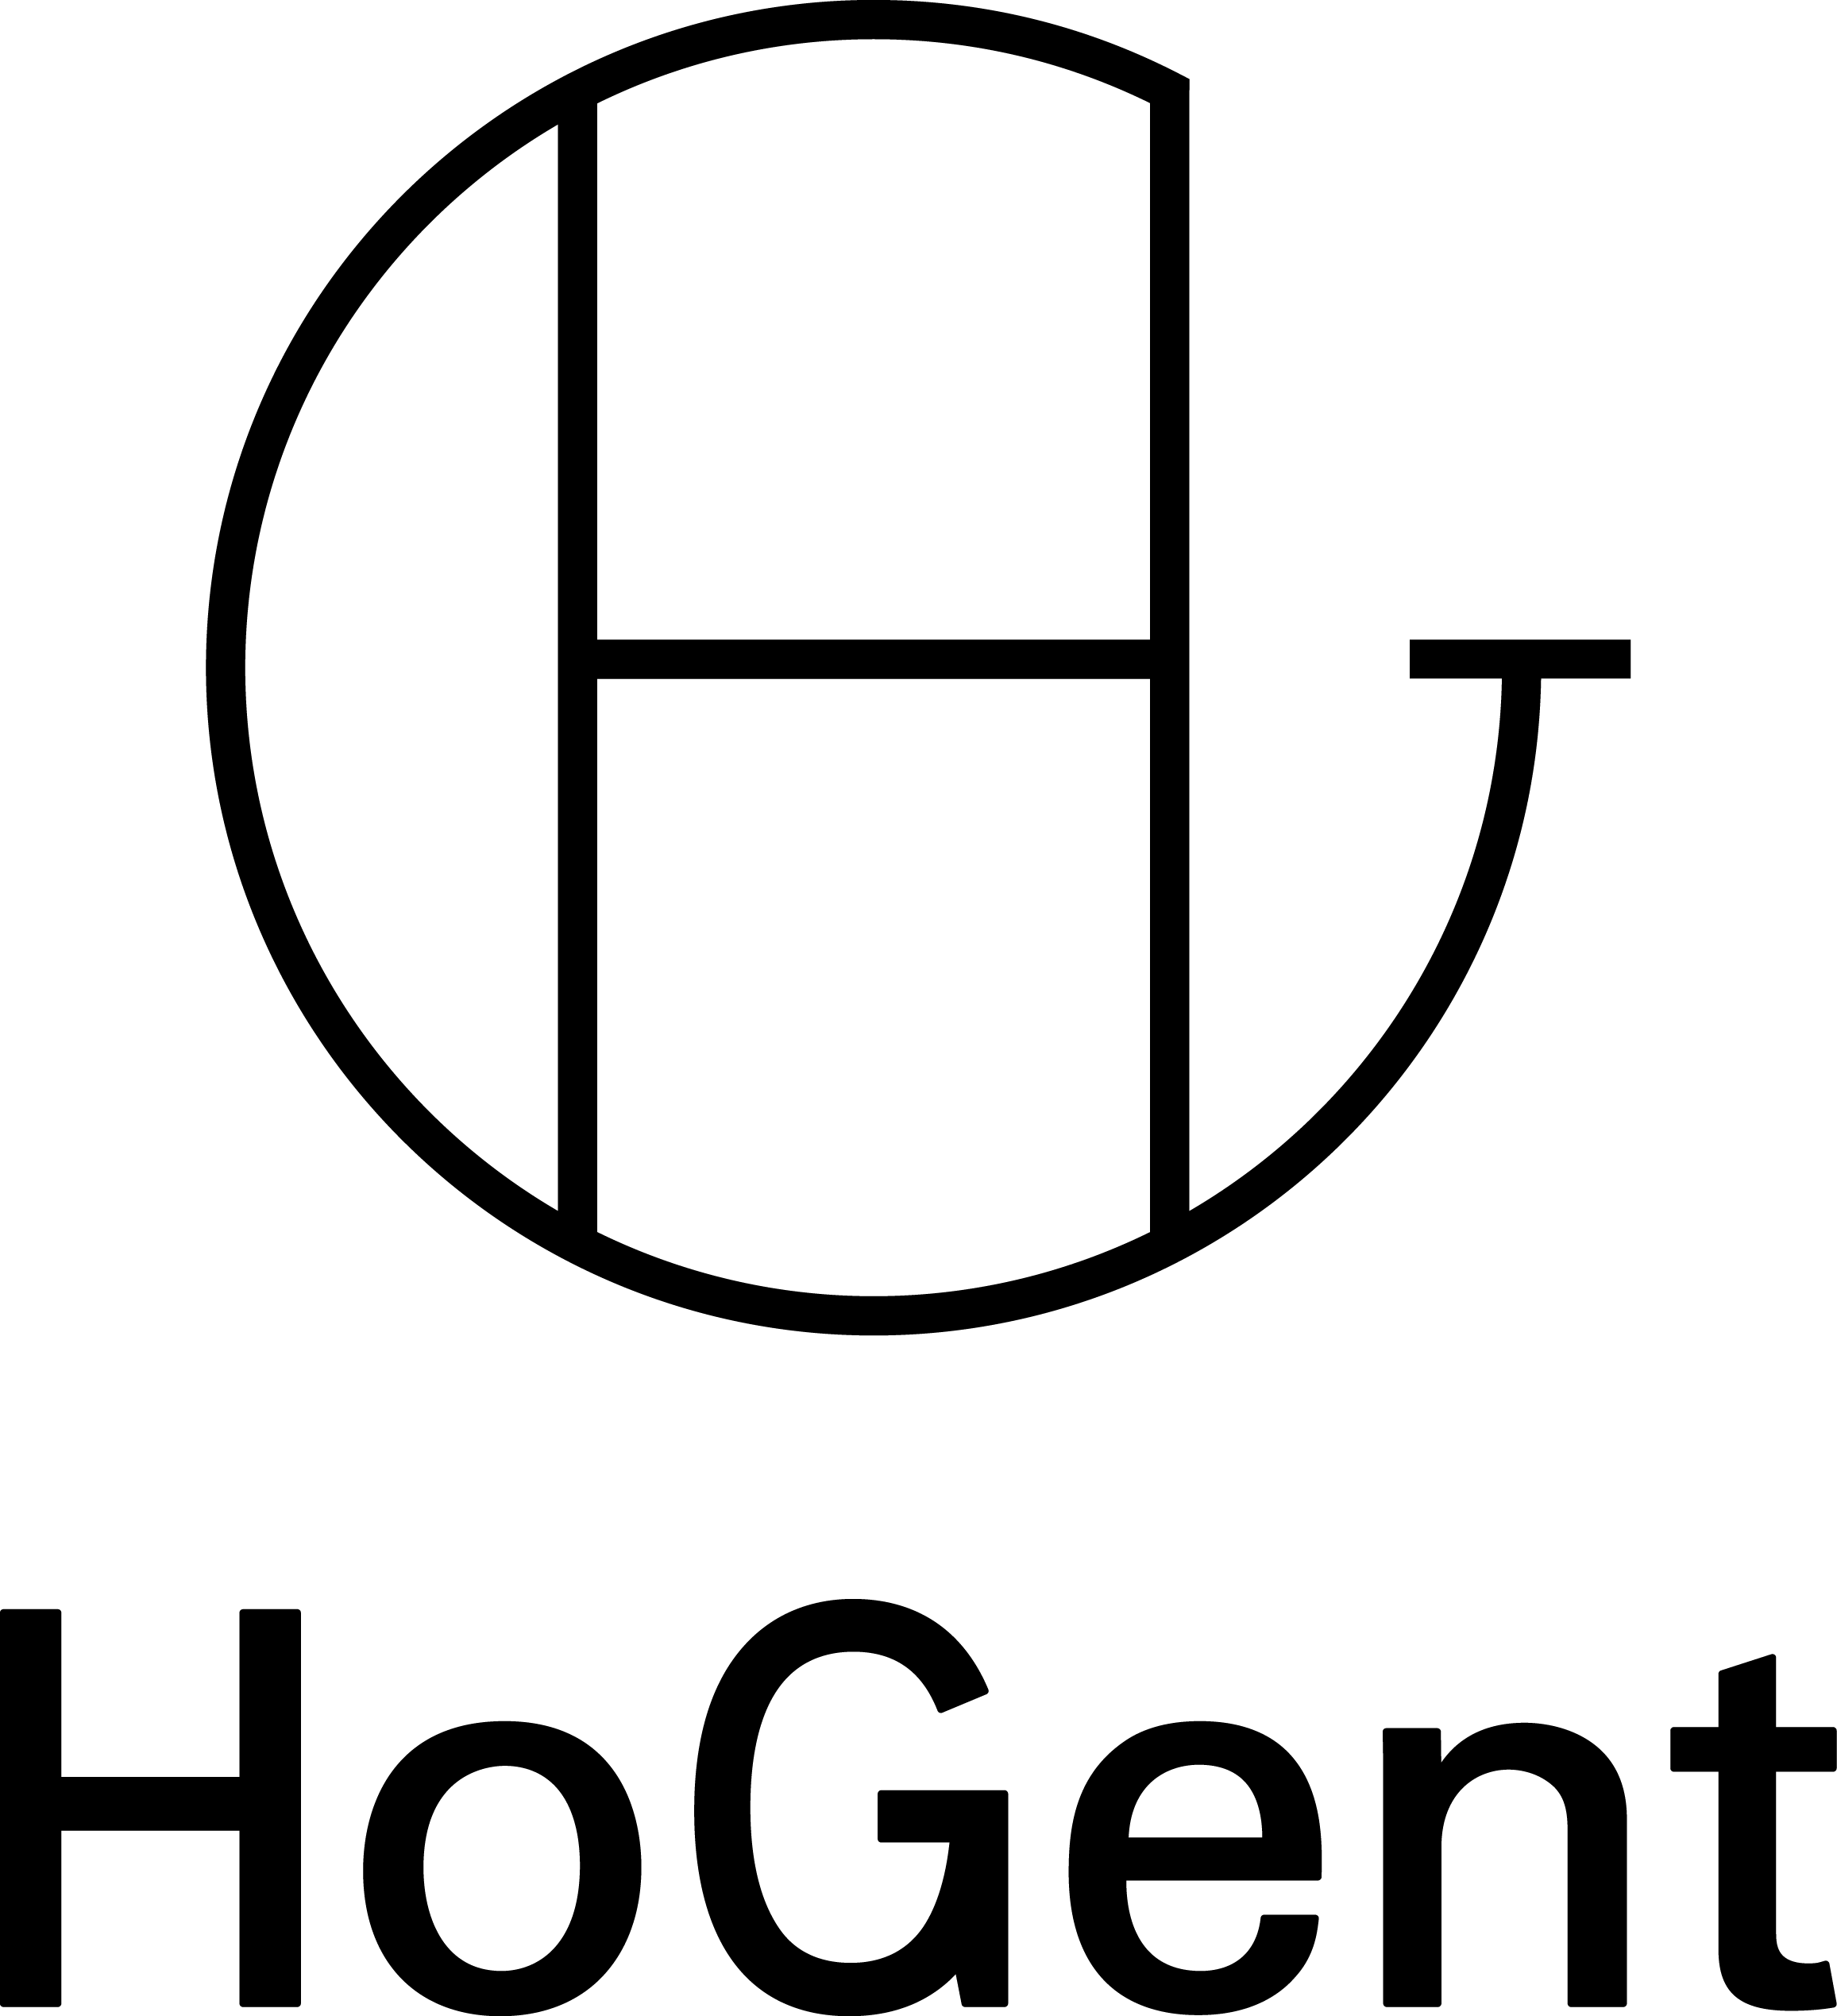
\includegraphics[width=2.5cm]{img/HG-beeldmerk-woordmerk}\\[.5cm]
    Faculteit Bedrijf en Organisatie\\[3cm]
    \titel
    \vfill
    \student\\[3.5cm]
    Scriptie voorgedragen tot het bekomen van de graad van\\professionele bachelor in de toegepaste informatica\\[2cm]
    Promotor:\\
    \promotor\\
    \ifdefempty{\copromotor}{\vspace{2.5cm}}{Co-promotor:\\\copromotor\\[2.5cm]}
    Instelling: \instelling\\[.5cm]
    Academiejaar: \academiejaar\\[.5cm]
    \ifcase \examenperiode \or Eerste \or Tweede \else Derde \fi examenperiode
    \endgroup

  \end{center}
  \restoregeometry
\end{titlepage}
  \emptypage
\begin{titlepage}
  \newgeometry{top=5.35cm,bottom=1.5cm,left=1.5cm,right=1.5cm}
  \begin{center}

    \begingroup
    \rmfamily
    \IfLanguageName{dutch}{Faculteit Bedrijf en Organisatie}{Faculty of Business and Information Management}\\[3cm]
    \titel
    \vfill
    \student\\[3.5cm]
    \IfLanguageName{dutch}{Scriptie voorgedragen tot het bekomen van de graad van\\professionele bachelor in de toegepaste informatica}{Thesis submitted in partial fulfillment of the requirements for the degree of\\professional bachelor of applied computer science}\\[2cm]
    Promotor:\\
    \promotor\\
    \ifdefempty{\copromotor}{\vspace{2.5cm}}{Co-promotor:\\\copromotor\\[2.5cm]}
    \IfLanguageName{dutch}{Instelling}{Institution}: \instelling\\[.5cm]
    \IfLanguageName{dutch}{Academiejaar}{Academic year}: \academiejaar\\[.5cm]
    \IfLanguageName{dutch}{%
    \ifcase \examenperiode \or Eerste \or Tweede \else Derde \fi examenperiode}{%
    \ifcase \examenperiode \or First \or Second \else Third \fi examination period}
    \endgroup

  \end{center}
  \restoregeometry
\end{titlepage}
}

%----------------------------------------------------------------------------------------
%	BIBLIOGRAPHY AND INDEX
%----------------------------------------------------------------------------------------

\usepackage[style=apa,backend=biber]{biblatex}
\usepackage{csquotes}
\DeclareLanguageMapping{dutch}{dutch-apa}
\addbibresource{bachproef-tin.bib} % BibTeX bibliography file
\defbibheading{bibempty}{}

\usepackage{calc} % For simpler calculation - used for spacing the index letter headings correctly
\usepackage{makeidx} % Required to make an index
\makeindex % Tells LaTeX to create the files required for indexing

%----------------------------------------------------------------------------------------
%	MAIN TABLE OF CONTENTS
%----------------------------------------------------------------------------------------

\usepackage{titletoc} % Required for manipulating the table of contents

\contentsmargin{0cm} % Removes the default margin

% Part text styling
\titlecontents{part}[0cm]
{\addvspace{20pt}\centering\large\bfseries}
{}
{}
{}

% Chapter text styling
\titlecontents{chapter}[1.25cm] % Indentation
{\addvspace{12pt}\large\sffamily\bfseries} % Spacing and font options for chapters
{\color{maincolor!60}\contentslabel[\Large\thecontentslabel]{1.25cm}\color{maincolor}} % Chapter number
{\color{maincolor}}
{\color{maincolor!60}\normalsize\;\titlerule*[.5pc]{.}\;\thecontentspage} % Page number

% Section text styling
\titlecontents{section}[1.25cm] % Indentation
{\addvspace{3pt}\sffamily\bfseries} % Spacing and font options for sections
{\contentslabel[\thecontentslabel]{1.25cm}} % Section number
{}
{\hfill\color{black}\thecontentspage} % Page number
[]

% Subsection text styling
\titlecontents{subsection}[1.25cm] % Indentation
{\addvspace{1pt}\sffamily\small} % Spacing and font options for subsections
{\contentslabel[\thecontentslabel]{1.25cm}} % Subsection number
{}
{\ \titlerule*[.5pc]{.}\;\thecontentspage} % Page number
[]

% List of figures
\titlecontents{figure}[0em]
{\addvspace{-5pt}\sffamily}
{\thecontentslabel\hspace*{1em}}
{}
{\ \titlerule*[.5pc]{.}\;\thecontentspage}
[]

% List of tables
\titlecontents{table}[0em]
{\addvspace{-5pt}\sffamily}
{\thecontentslabel\hspace*{1em}}
{}
{\ \titlerule*[.5pc]{.}\;\thecontentspage}
[]

%----------------------------------------------------------------------------------------
%	MINI TABLE OF CONTENTS IN PART HEADS
%----------------------------------------------------------------------------------------

% Chapter text styling
\titlecontents{lchapter}[0em] % Indenting
{\addvspace{15pt}\large\sffamily\bfseries} % Spacing and font options for chapters
{\color{maincolor}\contentslabel[\Large\thecontentslabel]{1.25cm}\color{maincolor}} % Chapter number
{}
{\color{maincolor}\normalsize\sffamily\bfseries\;\titlerule*[.5pc]{.}\;\thecontentspage} % Page number

% Section text styling
\titlecontents{lsection}[0em] % Indenting
{\sffamily\small} % Spacing and font options for sections
{\contentslabel[\thecontentslabel]{1.25cm}} % Section number
{}
{}

% Subsection text styling
\titlecontents{lsubsection}[.5em] % Indentation
{\normalfont\footnotesize\sffamily} % Font settings
{}
{}
{}

%----------------------------------------------------------------------------------------
%	PAGE HEADERS
%----------------------------------------------------------------------------------------

\usepackage{fancyhdr} % Required for header and footer configuration

\pagestyle{fancy}
\renewcommand{\chaptermark}[1]{\markboth{\sffamily\normalsize\bfseries\chaptername\ \thechapter.\ #1}{}} % Chapter text font settings
\renewcommand{\sectionmark}[1]{\markright{\sffamily\normalsize\thesection\hspace{5pt}#1}{}} % Section text font settings
\fancyhf{} \fancyhead[LE,RO]{\sffamily\normalsize\thepage} % Font setting for the page number in the header
\fancyhead[LO]{\rightmark} % Print the nearest section name on the left side of odd pages
\fancyhead[RE]{\leftmark} % Print the current chapter name on the right side of even pages
\renewcommand{\headrulewidth}{0.5pt} % Width of the rule under the header
\addtolength{\headheight}{2.5pt} % Increase the spacing around the header slightly
\renewcommand{\footrulewidth}{0pt} % Removes the rule in the footer
\fancypagestyle{plain}{\fancyhead{}\renewcommand{\headrulewidth}{0pt}} % Style for when a plain pagestyle is specified

% Removes the header from odd empty pages at the end of chapters
\makeatletter
\renewcommand{\cleardoublepage}{
\clearpage\ifodd\c@page\else
\hbox{}
\vspace*{\fill}
\thispagestyle{empty}
\newpage
\fi}

%----------------------------------------------------------------------------------------
%	THEOREM STYLES
%----------------------------------------------------------------------------------------

\usepackage{amsmath,amsfonts,amssymb,amsthm} % For math equations, theorems, symbols, etc

\newcommand{\intoo}[2]{\mathopen{]}#1\,;#2\mathclose{[}}
\newcommand{\ud}{\mathop{\mathrm{{}d}}\mathopen{}}
\newcommand{\intff}[2]{\mathopen{[}#1\,;#2\mathclose{]}}
\newtheorem{notation}{Notation}[chapter]

% Boxed/framed environments
\newtheoremstyle{maincolornumbox}% % Theorem style name
{0pt}% Space above
{0pt}% Space below
{\normalfont}% % Body font
{}% Indent amount
{\small\bf\sffamily\color{maincolor}}% % Theorem head font
{\;}% Punctuation after theorem head
{0.25em}% Space after theorem head
{\small\sffamily\color{maincolor}\thmname{#1}\nobreakspace\thmnumber{\@ifnotempty{#1}{}\@upn{#2}}% Theorem text (e.g. Theorem 2.1)
\thmnote{\nobreakspace\the\thm@notefont\sffamily\bfseries\color{black}---\nobreakspace#3.}} % Optional theorem note
\renewcommand{\qedsymbol}{$\blacksquare$}% Optional qed square

\newtheoremstyle{blacknumex}% Theorem style name
{5pt}% Space above
{5pt}% Space below
{\normalfont}% Body font
{} % Indent amount
{\small\bf\sffamily}% Theorem head font
{\;}% Punctuation after theorem head
{0.25em}% Space after theorem head
{\small\sffamily{\tiny\ensuremath{\blacksquare}}\nobreakspace\thmname{#1}\nobreakspace\thmnumber{\@ifnotempty{#1}{}\@upn{#2}}% Theorem text (e.g. Theorem 2.1)
\thmnote{\nobreakspace\the\thm@notefont\sffamily\bfseries---\nobreakspace#3.}}% Optional theorem note

\newtheoremstyle{blacknumbox} % Theorem style name
{0pt}% Space above
{0pt}% Space below
{\normalfont}% Body font
{}% Indent amount
{\small\bf\sffamily}% Theorem head font
{\;}% Punctuation after theorem head
{0.25em}% Space after theorem head
{\small\sffamily\thmname{#1}\nobreakspace\thmnumber{\@ifnotempty{#1}{}\@upn{#2}}% Theorem text (e.g. Theorem 2.1)
\thmnote{\nobreakspace\the\thm@notefont\sffamily\bfseries---\nobreakspace#3.}}% Optional theorem note

% Non-boxed/non-framed environments
\newtheoremstyle{maincolornum}% % Theorem style name
{5pt}% Space above
{5pt}% Space below
{\normalfont}% % Body font
{}% Indent amount
{\small\bf\sffamily\color{maincolor}}% % Theorem head font
{\;}% Punctuation after theorem head
{0.25em}% Space after theorem head
{\small\sffamily\color{maincolor}\thmname{#1}\nobreakspace\thmnumber{\@ifnotempty{#1}{}\@upn{#2}}% Theorem text (e.g. Theorem 2.1)
\thmnote{\nobreakspace\the\thm@notefont\sffamily\bfseries\color{black}---\nobreakspace#3.}} % Optional theorem note
\renewcommand{\qedsymbol}{$\blacksquare$}% Optional qed square
\makeatother

% Defines the theorem text style for each type of theorem to one of the three styles above
\newcounter{dummy}
\numberwithin{dummy}{section}
\theoremstyle{maincolornumbox}
\newtheorem{theoremeT}[dummy]{Theorem}
\newtheorem{problem}{Problem}[chapter]
\newtheorem{exerciseT}{Exercise}[chapter]
\theoremstyle{blacknumex}
\newtheorem{exampleT}{Example}[chapter]
\theoremstyle{blacknumbox}
\newtheorem{vocabulary}{Vocabulary}[chapter]
\newtheorem{definitionT}{Definition}[section]
\newtheorem{corollaryT}[dummy]{Corollary}
\theoremstyle{maincolornum}
\newtheorem{proposition}[dummy]{Proposition}

%----------------------------------------------------------------------------------------
%	DEFINITION OF COLORED BOXES
%----------------------------------------------------------------------------------------

\RequirePackage[framemethod=default]{mdframed} % Required for creating the theorem, definition, exercise and corollary boxes

% Theorem box
\newmdenv[skipabove=7pt,
skipbelow=7pt,
backgroundcolor=black!5,
linecolor=maincolor,
innerleftmargin=5pt,
innerrightmargin=5pt,
innertopmargin=5pt,
leftmargin=0cm,
rightmargin=0cm,
innerbottommargin=5pt]{tBox}

% Exercise box
\newmdenv[skipabove=7pt,
skipbelow=7pt,
rightline=false,
leftline=true,
topline=false,
bottomline=false,
backgroundcolor=maincolor!10,
linecolor=maincolor,
innerleftmargin=5pt,
innerrightmargin=5pt,
innertopmargin=5pt,
innerbottommargin=5pt,
leftmargin=0cm,
rightmargin=0cm,
linewidth=4pt]{eBox}

% Definition box
\newmdenv[skipabove=7pt,
skipbelow=7pt,
rightline=false,
leftline=true,
topline=false,
bottomline=false,
linecolor=maincolor,
innerleftmargin=5pt,
innerrightmargin=5pt,
innertopmargin=0pt,
leftmargin=0cm,
rightmargin=0cm,
linewidth=4pt,
innerbottommargin=0pt]{dBox}

% Corollary box
\newmdenv[skipabove=7pt,
skipbelow=7pt,
rightline=false,
leftline=true,
topline=false,
bottomline=false,
linecolor=gray,
backgroundcolor=black!5,
innerleftmargin=5pt,
innerrightmargin=5pt,
innertopmargin=5pt,
leftmargin=0cm,
rightmargin=0cm,
linewidth=4pt,
innerbottommargin=5pt]{cBox}

% Creates an environment for each type of theorem and assigns it a theorem text style from the "Theorem Styles" section above and a colored box from above
\newenvironment{theorem}{\begin{tBox}\begin{theoremeT}}{\end{theoremeT}\end{tBox}}
\newenvironment{exercise}{\begin{eBox}\begin{exerciseT}}{\hfill{\color{maincolor}\tiny\ensuremath{\blacksquare}}\end{exerciseT}\end{eBox}}
\newenvironment{definition}{\begin{dBox}\begin{definitionT}}{\end{definitionT}\end{dBox}}
\newenvironment{example}{\begin{exampleT}}{\hfill{\tiny\ensuremath{\blacksquare}}\end{exampleT}}
\newenvironment{corollary}{\begin{cBox}\begin{corollaryT}}{\end{corollaryT}\end{cBox}}

%----------------------------------------------------------------------------------------
%	REMARK ENVIRONMENT
%----------------------------------------------------------------------------------------

\newenvironment{remark}{\par\vspace{10pt}\small % Vertical white space above the remark and smaller font size
\begin{list}{}{
\leftmargin=35pt % Indentation on the left
\rightmargin=25pt}\item\ignorespaces % Indentation on the right
\makebox[-2.5pt]{\begin{tikzpicture}[overlay]
\node[draw=maincolor!60,line width=1pt,circle,fill=maincolor!25,font=\sffamily\bfseries,inner sep=2pt,outer sep=0pt] at (-15pt,0pt){\textcolor{maincolor}{R}};\end{tikzpicture}} % Orange R in a circle
\advance\baselineskip -1pt}{\end{list}\vskip5pt} % Tighter line spacing and white space after remark

%----------------------------------------------------------------------------------------
%	SECTION NUMBERING IN THE MARGIN
%----------------------------------------------------------------------------------------

\makeatletter
\renewcommand{\@seccntformat}[1]{\llap{\textcolor{maincolor}{\csname the#1\endcsname}\hspace{1em}}}
\renewcommand{\section}{\@startsection{section}{1}{\z@}
{-4ex \@plus -1ex \@minus -.4ex}
{1ex \@plus.2ex }
{\normalfont\large\sffamily\bfseries}}
\renewcommand{\subsection}{\@startsection {subsection}{2}{\z@}
{-3ex \@plus -0.1ex \@minus -.4ex}
{0.5ex \@plus.2ex }
{\normalfont\sffamily\bfseries}}
\renewcommand{\subsubsection}{\@startsection {subsubsection}{3}{\z@}
{-2ex \@plus -0.1ex \@minus -.2ex}
{.2ex \@plus.2ex }
{\normalfont\small\sffamily\bfseries}}
\renewcommand\paragraph{\@startsection{paragraph}{4}{\z@}
{-2ex \@plus-.2ex \@minus .2ex}
{.1ex}
{\normalfont\small\sffamily\bfseries}}

%----------------------------------------------------------------------------------------
%	PART HEADINGS
%----------------------------------------------------------------------------------------

% numbered part in the table of contents
\newcommand{\@mypartnumtocformat}[2]{%
\setlength\fboxsep{0pt}%
\noindent\colorbox{maincolor!20}{\strut\parbox[c][.7cm]{\ecart}{\color{maincolor!70}\Large\sffamily\bfseries\centering#1}}\hskip\esp\colorbox{maincolor!40}{\strut\parbox[c][.7cm]{\linewidth-\ecart-\esp}{\Large\sffamily\centering#2}}}%
%%%%%%%%%%%%%%%%%%%%%%%%%%%%%%%%%%
% unnumbered part in the table of contents
\newcommand{\@myparttocformat}[1]{%
\setlength\fboxsep{0pt}%
\noindent\colorbox{maincolor!40}{\strut\parbox[c][.7cm]{\linewidth}{\Large\sffamily\centering#1}}}%
%%%%%%%%%%%%%%%%%%%%%%%%%%%%%%%%%%
\newlength\esp
\setlength\esp{4pt}
\newlength\ecart
\setlength\ecart{1.2cm-\esp}
\newcommand{\thepartimage}{}%
\newcommand{\partimage}[1]{\renewcommand{\thepartimage}{#1}}%
\def\@part[#1]#2{%
\ifnum \c@secnumdepth >-2\relax%
\refstepcounter{part}%
\addcontentsline{toc}{part}{\texorpdfstring{\protect\@mypartnumtocformat{\thepart}{#1}}{\partname~\thepart\ ---\ #1}}
\else%
\addcontentsline{toc}{part}{\texorpdfstring{\protect\@myparttocformat{#1}}{#1}}%
\fi%
\startcontents%
\markboth{}{}%
{\thispagestyle{empty}%
\begin{tikzpicture}[remember picture,overlay]%
\node at (current page.north west){\begin{tikzpicture}[remember picture,overlay]%
\fill[maincolor!20](0cm,0cm) rectangle (\paperwidth,-\paperheight);
\node[anchor=north] at (4cm,-3.25cm){\color{maincolor!40}\fontsize{220}{100}\sffamily\bfseries\@Roman\c@part};
\node[anchor=south east] at (\paperwidth-1cm,-\paperheight+1cm){\parbox[t][][t]{8.5cm}{
\printcontents{l}{0}{\setcounter{tocdepth}{1}}%
}};
\node[anchor=north east] at (\paperwidth-1.5cm,-3.25cm){\parbox[t][][t]{15cm}{\strut\raggedleft\color{white}\fontsize{30}{30}\sffamily\bfseries#2}};
\end{tikzpicture}};
\end{tikzpicture}}%
\@endpart}
\def\@spart#1{%
\startcontents%
\phantomsection
{\thispagestyle{empty}%
\begin{tikzpicture}[remember picture,overlay]%
\node at (current page.north west){\begin{tikzpicture}[remember picture,overlay]%
\fill[maincolor!20](0cm,0cm) rectangle (\paperwidth,-\paperheight);
\node[anchor=north east] at (\paperwidth-1.5cm,-3.25cm){\parbox[t][][t]{15cm}{\strut\raggedleft\color{white}\fontsize{30}{30}\sffamily\bfseries#1}};
\end{tikzpicture}};
\end{tikzpicture}}
\addcontentsline{toc}{part}{\texorpdfstring{%
\setlength\fboxsep{0pt}%
\noindent\protect\colorbox{maincolor!40}{\strut\protect\parbox[c][.7cm]{\linewidth}{\Large\sffamily\protect\centering #1\quad\mbox{}}}}{#1}}%
\@endpart}
\def\@endpart{\vfil\newpage
\if@twoside
\if@openright
\null
\thispagestyle{empty}%
\newpage
\fi
\fi
\if@tempswa
\twocolumn
\fi}

%----------------------------------------------------------------------------------------
%	CHAPTER HEADINGS
%----------------------------------------------------------------------------------------

% A switch to conditionally include a picture, implemented by  Christian Hupfer
\newif\ifusechapterimage
\usechapterimagetrue
\newcommand{\thechapterimage}{}%
\newcommand{\chapterimage}[1]{\ifusechapterimage\renewcommand{\thechapterimage}{#1}\fi}%
\def\@makechapterhead#1{%
{\parindent \z@ \raggedright \normalfont
\ifnum \c@secnumdepth >\m@ne
\if@mainmatter
\begin{tikzpicture}[remember picture,overlay]
\node at (current page.north west)
{\begin{tikzpicture}[remember picture,overlay]
\node[anchor=north west,inner sep=0pt] at (0,0) {\ifusechapterimage\includegraphics[width=\paperwidth]{\thechapterimage}\fi};
\draw[anchor=west] (\Gm@lmargin,-9cm) node [line width=2pt,rounded corners=15pt,draw=maincolor,fill=white,fill opacity=0.5,inner sep=15pt]{\strut\makebox[22cm]{}};
\draw[anchor=west] (\Gm@lmargin+.3cm,-9cm) node {\huge\sffamily\bfseries\color{black}\thechapter. #1\strut};
\end{tikzpicture}};
\end{tikzpicture}
\else
\begin{tikzpicture}[remember picture,overlay]
\node at (current page.north west)
{\begin{tikzpicture}[remember picture,overlay]
\node[anchor=north west,inner sep=0pt] at (0,0) {\ifusechapterimage\includegraphics[width=\paperwidth]{\thechapterimage}\fi};
\draw[anchor=west] (\Gm@lmargin,-9cm) node [line width=2pt,rounded corners=15pt,draw=maincolor,fill=white,fill opacity=0.5,inner sep=15pt]{\strut\makebox[22cm]{}};
\draw[anchor=west] (\Gm@lmargin+.3cm,-9cm) node {\huge\sffamily\bfseries\color{black}#1\strut};
\end{tikzpicture}};
\end{tikzpicture}
\fi\fi\par\vspace*{270\p@}}}

%-------------------------------------------

\def\@makeschapterhead#1{%
\begin{tikzpicture}[remember picture,overlay]
\node at (current page.north west)
{\begin{tikzpicture}[remember picture,overlay]
\node[anchor=north west,inner sep=0pt] at (0,0) {\ifusechapterimage\includegraphics[width=\paperwidth]{\thechapterimage}\fi};
\draw[anchor=west] (\Gm@lmargin,-9cm) node [line width=2pt,rounded corners=15pt,draw=maincolor,fill=white,fill opacity=0.5,inner sep=15pt]{\strut\makebox[22cm]{}};
\draw[anchor=west] (\Gm@lmargin+.3cm,-9cm) node {\huge\sffamily\bfseries\color{black}#1\strut};
\end{tikzpicture}};
\end{tikzpicture}
\par\vspace*{270\p@}}
\makeatother

%----------------------------------------------------------------------------------------
%	HYPERLINKS IN THE DOCUMENTS
%----------------------------------------------------------------------------------------

\usepackage{hyperref}
\hypersetup{hidelinks,backref=true,pagebackref=true,hyperindex=true,colorlinks=false,breaklinks=true,urlcolor= maincolor,bookmarks=true,bookmarksopen=false,pdftitle={Title},pdfauthor={Author}}
\usepackage{bookmark}
\bookmarksetup{
open,
numbered,
addtohook={%
\ifnum\bookmarkget{level}=0 % chapter
\bookmarksetup{bold}%
\fi
\ifnum\bookmarkget{level}=-1 % part
\bookmarksetup{color=maincolor,bold}%
\fi
}
}

%----------------------------------------------------------------------------------------
%	Java source code
%----------------------------------------------------------------------------------------

% Commando voor invoegen Java-broncodebestanden (dank aan Niels Corneille)
% Gebruik:
%   \codefragment{source/MijnKlasse.java}{Uitleg bij de code}
%
% Je kan dit aanpassen aan de taal die je zelf het meeste gebruikt in je
% bachelorproef.
\newcommand{\codefragment}[2]{ \lstset{%
  language=java,
  breaklines=true,
  float=th,
  caption={#2},
  basicstyle=\scriptsize,
  frame=single,
  extendedchars=\true
}
\lstinputlisting{#1}}

% Leeg blad
\newcommand{\emptypage}{%
\newpage
\thispagestyle{empty}
\mbox{}
\newpage
}


%%---------- Documenteigenschappen --------------------------------------------
%% TODO: Vul dit aan met je eigen info:

% Je eigen naam
\newcommand{\student}{Simon Jang}

% De naam van je promotor (lector van de opleiding)
\newcommand{\promotor}{Stefaan De Cock}

% De naam van je co-promotor. Als je promotor ook je opdrachtgever is en je
% dus ook inhoudelijk begeleidt (en enkel dan!), mag je dit leeg laten.
\newcommand{\copromotor}{Sam Verschueren}

% Indien je bachelorproef in opdracht van/in samenwerking met een bedrijf of
% externe organisatie geschreven is, geef je hier de naam. Zoniet laat je dit
% zoals het is.
\newcommand{\instelling}{Pridiktiv.care - Into.care}

% De titel van het rapport/bachelorproef
\newcommand{\titel}{Opslag en synchronisatie van offline data bij mobiele applicaties}

% Datum van indienen (gebruik telkens de deadline, ook al geef je eerder af)
\newcommand{\datum}{27 mei 2017}

% Academiejaar
\newcommand{\academiejaar}{2016-2017}

% Examenperiode
%  - 1e semester = 1e examenperiode => 1
%  - 2e semester = 2e examenperiode => 2
%  - tweede zit  = 3e examenperiode => 3
\newcommand{\examenperiode}{2}

%%=============================================================================
%% Inhoud document
%%=============================================================================

\begin{document}

%---------- Taalselectie ------------------------------------------------------
%% Als je je bachelorproef in het Engels schrijft, haal dan onderstaande regel
%% uit commentaar. Let op: de tekst op de voorkaft blijft in het Nederlands, en
%% dat is ook de bedoeling!
%\selectlanguage{english}

%---------- Titelblad ---------------------------------------------------------
\inserttitlepage

%---------- Samenvatting, voorwoord -------------------------------------------
\usechapterimagefalse
%%=============================================================================
%% Samenvatting
%%=============================================================================

%% TODO: De "abstract" of samenvatting is een kernachtige (~ 1 blz. voor een
%% thesis) synthese van het document.
%%
%% Deze aspecten moeten zeker aan bod komen:
%% - Context: waarom is dit werk belangrijk?
%% - Nood: waarom moest dit onderzocht worden?
%% - Taak: wat heb je precies gedaan?
%% - Object: wat staat in dit document geschreven?
%% - Resultaat: wat was het resultaat?
%% - Conclusie: wat is/zijn de belangrijkste conclusie(s)?
%% - Perspectief: blijven er nog vragen open die in de toekomst nog kunnen
%%    onderzocht worden? Wat is een mogelijk vervolg voor jouw onderzoek?
%%
%% LET OP! Een samenvatting is GEEN voorwoord!

\IfLanguageName{english}{%
\selectlanguage{dutch}
\chapter*{Samenvatting}
\lipsum[1-4]
\selectlanguage{english}
}{}

%%---------- Samenvatting -----------------------------------------------------
%%
%% De samenvatting in de hoofdtaal van het document

\chapter*{\IfLanguageName{dutch}{Samenvatting}{Abstract}}

Mobiele applicatieontwikkeling beschouwt toegang tot internet vaak als vanzelfsprekend wanneer een mobiele applicatie wordt gebruikt. Dit is echter niet het geval in elke (werk)omgeving. Daarom moet de ontwikkelaar ervoor zorgen dat de applicatie de data ook lokaal kan opslaan indien de wijzigingen niet meteen kunnen worden doorgevoerd naar de achterliggende infrastructuur. Dit probleem vormt voor ontwikkelaars een uitdaging omdat de data integriteit moet worden gewaarborgd wanneer het toestel terug verbonden is met het Internet. Het gebruik van een performante en betrouwbare methode voor de data die offline wordt ingegeven te synchroniseren met de online cloud-based databank is dus essentieel. Hierbij is het belangrijk om een onderscheid te maken tussen use cases waarbij de developer gebruik maakt van fully-managed databases zoals onder andere DynamoDB van Amazon Web Services en use cases waarbij men zelf de database(s) beheert op verschillende virtuele machines. In het onderzoek is synchronisatie specifiek onderzocht voor de fully-managed database DynamoDB, een backend die gebruikt maakt van een serverless microservices architectuur en een Angular applicatie als client applicatie. 

Na onderzoek en reserach is gebleken dat er verschillende manieren van synchronisatie zijn. Technologie\"en als CouchDB en Firebase automatiseren het synchronisatieproces. Maar wanneer men zelf de synchronisatie wenst te realiseren is het belangrijk om de verschillende use cases onder te verdelen volgens synchronisatie methode en zo verder te werken. Er zijn scenario's waar er geen conflicten zijn maar performantie de belangrijkste factor is bv. Read-Only Optimised. Wanneer er conflicten optreden kan men dan kiezen voor First Write Wins of Last Write Wins waarbij er onvermijdelijk data verloren gaat of andere strategie\"en van conflict resolution. Caching speelt een belangrijke rol in de transitie van online naar offline en synchronisatie is belangrijk bij de overgang van offline naar online. Met behulp van caching en synchronisatie is het mogelijk om een robuuste applicatie te ontwikkelen waarbij data integriteit en functionaliteit worden gegarandeerd.
%%=============================================================================
%% Voorwoord
%%=============================================================================

\chapter*{Voorwoord}
\label{ch:voorwoord}

%% TODO:
%% Het voorwoord is het enige deel van de bachelorproef waar je vanuit je
%% eigen standpunt (``ik-vorm'') mag schrijven. Je kan hier bv. motiveren
%% waarom jij het onderwerp wil bespreken.
%% Vergeet ook niet te bedanken wie je geholpen/gesteund/... heeft

Mijn interesse in mobiele- en web applicaties was voor mij de reden om de opleiding Toegepaste Informatica aan de Hogeschool Gent te starten. Deze bachelorproef vormt het sluitstuk in mijn opleiding en de keuze van het onderwerp is tot stand gekomen door de samenwerking met mijn stageplaats Pridiktiv.care - Into.care. Er was nood aan een onderzoek naar offline data opslag en synchronisatie bij hun mobiele applicatie. Met de groei van IoT en de digitalisering binnen verschillende sectoren, lijkt offline / online synchronisatie relevanter dan ooit.

Het schrijven van een bachelorpaper is geen eenvoudige opdracht en ik zou daarom enkele personen willen bedanken voor hun ondersteuning en expertise. Eerst en vooral wil ik mijn co-promotor en stage-mentor Sam Verschueren bedanken voor zijn inzet en geduld bij de talloze vragen die ik het gesteld in verband met web applicaties. Daarnaast ben ik ook zeer dankbaar voor de intense begeleiding en feedback die ik heb ontvangen van mijn promotor Stefaan De Cock. Tenslotte wil ook mijn partner en vrienden bedanken voor de hulp die ze hebben aangeboden bij het lezen van mijn bachelorproef en de morele ondersteuning.

%---------- Inhoudstafel ------------------------------------------------------
\pagestyle{empty} % No headers
\tableofcontents % Print the table of contents itself
\cleardoublepage % Forces the first chapter to start on an odd page so it's on the right
\pagestyle{fancy} % Print headers again

%---------- Lijst afkortingen, termen -----------------------------------------
%% Als je een lijst van afkortingen of termen wil toevoegen, dan hoort die
%% hier thuis. Gebruik bijvoorbeeld de ``glossaries'' package.
%%=============================================================================
%% Glossarium
%%=============================================================================

\chapter{Glossarium}
\label{ch:glossarium}

%% TODO: Woordenlijst met alle begrippen

\begin{description}
\item[Single-Page Application, SPA] \hfill \ Een single-page application (SPA) is een web applicatie of website waarbij noodzakelijke HTML, CSS en JavaScript dynamisch wordt ingeladen of bij de eerste page load, afhankelijk van de acties van de gebruiker. De volledige pagina wordt bij een SPA nooit volledig herladen. Het is wel mogelijk dat onderdelen van de pagina dynamisch wordt gewijzigd. De data van de SPA wordt dynamisch opgevraagd van de web server. 
\item[Single Source Of Truth, SSOT] \hfill \ In de context van het ontwerp van informatica systemen is de single source of truth een techniek of informatie en data structuren op een bepaalde manier te structureren zodat die niet gedupliceerd wordt. Alle informatie wordt opgehaald in een centraal punt en dat is voor de applicatie en haar componenten de enige plaats waar die informatie kan worden opgehaald. Ngrx store vervult die rol in een Angular applicatie.
\item[Angular CLI] \hfill \ Angular CLI is een command line interface tool waarbij een volledige Angular project wordt gebouwd met minimale configuratie. Er wordt een basis structuur, tests, root module en root component aangemaakt. Met behulp van Webpack worden alle files dan gebundeld in enkele static files. Dankzij Angular CLI wordt er heel wat tijd uitgespaard omdat een groot deel van de configuratie wegvalt. Angular CLI wordt gebruikt de business case van Pridiktiv en in het prototype.
\end{description}

%%---------- Kern -------------------------------------------------------------

%%=============================================================================
%% Inleiding
%%=============================================================================
\chapter{Inleiding}
\label{ch:inleiding}
Het onderzoek zal verschillende methodes voor offline opslag en synchronisatie analyseren en onderzoeken. Het onderzoek zal van elke methode de voor- en nadelen overlopen en de toepassing tonen met behulp van een prototype. In de sectie 'Business Case' wordt de business case van Pridiktiv.care - Into.care toegelicht. Daarna worden in 'Terminologie' de verschillende relevante termen overlopen. In 'Stand van zaken' komt de context en noodzaak van het onderzoek aan bod. Tenslotte volgt de probleemstelling, de onderzoeksvraag en de opzet van de bachelorproef.
%% literatuurstudie. Vergeet niet telkens je bronnen te vermelden!
\section{Business Case}
\label{sec:business-case}
De business case van Pridiktiv vormt het vertrekpunt van deze studie en wordt nu nog wat verder toegelicht. De applicatie draait op een smartphone in een woonzorgcentrum. Het woonzorgcentrum beschikt over draadloos internet maar de dekking is niet het volledige gebouw. Hierdoor moet de applicatie ook offline werken. Wanneer verschillende waarden worden geregistreerd met de applicatie (zoals bloeddruk, gewicht, inname medicatie) worden die offline opgeslagen in een IndexedDB. Wanneer het toestel terug online komt, moeten deze waarden worden doorgestuurd naar de backend. Het is essentieel dat er geen data verloren gaat aangezien het gaat om medische data. Het huidige algoritme doet een HTTP call wanneer een waarde wordt ingegeven. Wanneer dit niet lukt, veronderstelt het algoritme dat de applicatie offline is en wordt de data lokaal opgeslagen. Wanneer het toestel terug online komt, dan worden de offline data gesynchroniseerd met de server. De realiteit wijst echter uit dat betrouwbaar internet eerder uitzonderlijk is in een woonzorgcentrum. In deze context is er dus nood aan een 'offline first' -  oplossing. De huidige applicatie is een Angular (het vroegere Angular 2) met ngrx als state container als een Cordova applicatie. Voor lokale opslag wordt momenteel gebruik gemaakt van Mozilla's LocalForage library. De backend maakt gebruik van Amazon Web Services met DynamoDB voor de persistentie van de data. Het is de intentie van dit onderzoek om te werken binnen het kader en de restricties van de business case. Indien een bepaalde methode of techniek niet van toepassing is voor de use case van Pridiktiv, wordt dit nadrukkelijk vermeld in de bachelorproef.
\section{Terminologie}
\label{sec:terminologie}
In deze sectie komen de verschillende begrippen met betrekking tot de componenten van het onderzoek, het prototype en tools aan bod. De volledige lijst met begrippen en termen kan u terugvinden onder het hoofdstuk 'Glossarium'. Er is een minimum kennis in verband met software ontwikkeling vereist van de lezer om deze sectie volledig te begrijpen.
\subsection{Huidige Web APIs voor lokale opslag}
Er zijn momenteel 4 APIs met betrekking lokale opslag die ondersteund worden door verschillende browsers. Deze APIs worden ondersteund door de Web Hypertext Application Technology Working Group, aangegeven door WHATWG en de specification van de API wordt dan gestandardiseerd door de World Wide Web Consortium, aangegeven door W3C. Dit proces is belangrijk omdat de APIs dan door de populaire browsers (Chrome, Firefox, Safari en Opera, Internet Explorer) worden ge\"integreerd. Op die manier kunnen webapplicaties gebruik maken van de verschillende APIs. Het is belangrijk om deze APIs kort te overlopen omdat ze steeds gebruikt worden bij de verschillende caching technieken om de data lokaal van web applicaties op te slaan.
\subsubsection{localStorage en sessionStorage}
Deze 2 APIs vallen onder Web Storage of DOM Storage. Wanneer de browser ondersteuning biedt voor Web Storage, zijn beide beschikbaar als een globaal object. Web Storage wordt vaak vergeleken met cookies. Terwijl die vergelijkbaar zijn in functie, verschilt web storage in volgende aspecten: 
\begin{itemize}  
\item Opslag ruimte: Afhankelijk van browser maar meestal 5 MB beschikbare opslagruimte in vergelijking met maar 4 kb voor cookies.
\item Client-side interface: Cookies kunnen zowel door server als client side worden gebruikt. Web storage valt exclusief onder client-side scripting.
\item Twee verschillende storage areas: localStorage en sessionStorage.
\item Een eenvoudigere programmeerbare interface in vergelijking met cookies.
\end{itemize}
\subsubsection{localStorage}
Data die in localStorage wordt opgeslagen is persistent tenzij die manueel wordt verwijderd door de gebruiker of applicatie. localStorage is dus een belangrijke kandidaat om data lokaal op te slaan in geval een applicatie offline moet kunnen worden gebruikt. Bij gevoelige data zoals medische data is het belangrijk om de data te verwijderen uit de localStorage wanneer die niet meer moet worden gecached.
\subsubsection{sessionStorage}
Het grote verschil met localStorage is dat sessionStorage een vervalttijd heeft en de inhoud van de sessionStorage wordt verwijderd wanneer de sessie vervalt. Een sessie vervalt bijvoorbeeld hij het openen van een nieuw tabblad of browser venster. Refreshen van de browser heeft geen impact op de sessionStorage. sessionStorage laat toe om instances van een webapplicatie te runnen in verschillende browser windows, zonder dat er conflicten optreden.
\subsubsection{lndexedDB}
IndexedDB is een Web API die gebruikt wordt het opslaan van relatief grote data structuren in browsers. Dankzij indexering is het mogelijk om snel en performant te zoeken in de databank. Net zoals SQL-databanken is IndexedDB een transactional database system. Het grote verschil is echter het gebruik van JSON objecten in plaats van fixed columns tables om data op te slaan, vergelijkbaar met andere NoSQL databanken zoals MongoDB of CouchDB. Onder impuls van Mozilla wordt IndexedDB waarschijnlijk de alternatieve storage standaard voor het web in de nabije toekomst.
\subsubsection{Web SQL}
Net zoals bij IndexedDB biedt Web SQL toegang tot een databank waar data structuren kunnen worden opgeslagen. Met een SQL variant is het dan mogelijk om queries uit te voeren op de Web SQL database. Momenteel biedt enkel SQLite een database systeem voor Web SQL. W3C werkt momenteel niet meer verder aan de specificatie van Web SQL omdat er te weinig onafhankelijke implementaties zijn van Web SQL. 
\subsection{Scalable Angular Architecture}
Bij de start van de ontwikkeling van een Angular applicatie is het belangrijk om na te denken over de architectuur van de applicatie. Moderne SPA-technologie\"en zoals React en Angular maken gebruik van components. Een component is combinatie van HTML, JavaScript en optioneel CSS. Door alles in componenten onder te verdelen is het eenvoudiger om de applicatie te onderhouden omdat alle relevante data word gegroepeerd. Componenten zelf kunnen 'dumb' zijn als ze enkel data voorstellen of 'smart' wanneer te data opvragen of verwerken.
De dataflow tussen componenten is ook belangrijk om een beheersbare applicatie te bouwen. Zo communiceren child components enkel maar met hun parent en interageert een parent met een 'store' (.cfr 'ngrx store: een state container') aan de hand van acties. Wanneer de state van gewijzigd wordt in de store, dan wordt de volledige component tree opnieuw ge\"evalueerd. Een ander belangrijk aspect van een scalable SPA is het inperken van de communicatiemogelijkheden van smart components. Door het gebruik van een extra abstractie layer, zoals een model of sandbox, is het mogelijk om de communicatie te verwerken in de abstractielaag en op die manier een microservice te genereren die gemakkelijk kan worden refactored indien er aanpassingen moeten gebeuren.
\subsection{ngrx store: een state container}
ngrx store is een container die de state van de applicatie bijhoudt waarbij performantie en consistentie centraal staan. De ngrx store is de 'single source of truth', verder benoemd als SSOT, voor de applicatie en moet ervoor zorgen dat de data van alle componenten consistent is met elkaar en er geen duplicate data is. Alle updates aan de data worden eerste weggeschreven naar de store en daarna gecachet. In het geval dat de gebruiker toegang heeft tot internet wordt de data verstuurd naar de achterliggende systemen. Indien er geen of slechte internetverbinding is, krijgt de user de gecachte data te zien dankzij de SSOT. De ngrx store werkt met volgende principes:
\begin{itemize}  
\item De state is een single immutable data structure.
\item Actions initialiseren veranderingen in de state.
\item Pure functions verwerken actions om een 'nieuwe' state te cre\"een.
\item De state van de store wordt geraadpleegd als een Observable van state die op zijn beurt een observer is van actions.
\end{itemize}
\subsection{Reactive programming paradigm}
Het reactive programming paradigm is gebouwd rond veranderende data flows, waarbij een applicatie kan reageren op nieuwe of andere input. Dankzij de ReactiveX library is het mogelijk om in verschillende programmeertalen componenten van reactive programming te gebruiken. De library laat toe om asynchronous en event-based applicaties te ontwikkelen, die in real-time data kunnen manipuleren en tonen. Het breidt het Observer design pattern waarbij het mogelijk is om verschillende operators te 'chainen' met elkaar zonder rekening te houden met low level concerns zoals threading, synchronisatie, thread safety, concurrent data structures en blocking I/O. De RxJs library van ReactiveX is volledig ge\"integreerd in Angular en ngrx store. Met Promises was het reeds mogelijk om asynchroon te programmeren in JavaScript dus wat zijn de voordelen van RxJs ten opzicht van standaard JavaScript? Een Promise kan maar een single event afhandelen en kan niet worden gecancelled. Een Observable kan worden beschouwd als een stream van objecten waarop verschillende operatoren zoals map, reduce en filter kunnen worden op toegepast en is lazy van natuur.
\subsection{Offline First}
Een stroming binnen web development waarbij offline gebruik als de basis wordt beschouwd van de applicatie. Net zoals bij 'Progressive Enhancement' wordt online functionaliteit beschouwt als een extra laag van features die de applicatie kan aanbieden. Het idee is gegroeid vanuit de teleurstelling dat 'always online' omwille van technische, geografische, financi\"ele en praktische redenen nog niet haalbaar is voor de nabije toekomst.
\subsection{Amazon Web Services}
Om zo het onderzoek zo dicht mogelijk te laten aansluiten bij de use case van Pridiktiv, wordt er ook gebruikt gemaakt van bepaalde onderdelen binnen AWS. Volgende componenten komen aan bod verder in de bachelor paper:
\begin{itemize}
\item S3, Amazon Simple Storage Service: S3 voorziet een API doe gebruikt kan worden om data tot 5 terabyte op te slaan en op te halen. Via een unique key kan het object uit S3 worden gehaald. In de business case wordt S3 gebruikt voor de opslag van foto's.
\item Lambda: Met AWS Lambda is het mogelijk om 'functies' uit te voeren in de cloud dus zonder een specifieke server structuur op te bouwen. De input voor de functie kan worden geleverd door HTTP endpoints maar ook door andere AWS services. De output kan dan bijvoorbeeld worden gepersisteerd door DynamoDB of teruggestuurd worden naar de client.
\item Amazon SNS, Amazon Simple Notification Service: Een push notificatie service die toelaat om berichten te sturen naar mobile clients, email adressen of andere services. Met SNS is het onder andere mogelijk om polling van clients te vermijden.
\item DynamoDB: DynamoDB is een NoSQL key-value database van AWS en wordt gebruikt door de business case voor de data opslag. DynamoDB voorziet geen automatische synchronisatie met clients.
\end{itemize}
\section{Stand van zaken}
\label{sec:stand-van-zaken}
Wanneer een ontwikkelaar de end user van zijn web -of mobiele applicatie wil voorstellen, dan denkt hij vaak aan een user met dezelfde eigenschappen als zichzelf (laatste smartphone, up-to-date besturingssysteem,  snelle internet verbinding). De ontwikkelomgeving (snelle desktop/laptop met een betrouwbare en snelle internet verbinding) simuleert amper de omgeving van de end user. Ziet de realiteit er van de end user anders uit. Bepaalde omgevingsfactoren zoals bv. tunnels, trein en vliegtuig kunnen hebben een grote invloed op de betrouwbaarheid van de connectie. Het klassieke client - server model waarbij de client enkel maar als het ware een view is van de data die door de server wordt bijgehouden, is achterhaald, want elke onderbreking in de internet connectie zorgt ervoor dat de applicatie niet meer kan worden gebruikt. Dat is een scenario dat ten alle kosten moet worden vermeden. Meeste mobiele- en webapplicaties hebben twee momenten waarbij er problemen kunnen optreden door de status van de connectie:
\begin{enumerate}  
\item Client push request naar de server
\item Client pull van server / server push naar client
\end{enumerate}
Afhankelijk van wat de applicatie wil doen, zijn er verschillende opties:
\begin{itemize}  
\item De gebruiker al dan niet op de hoogte brengen van de veranderingen in de status van de connectie. Bijvoorbeeld: Bij het versturen van bericht, de gebruiker op de hoogte brengen dat het bericht pas wordt verstuurd wanneer de applicatie terug online is.
\item Offline client-side creatie en manipulatie van data toelaten aan de hand van caching en wanneer de applicatie terug online 
\item Uitschakelen of aanpassen van bepaalde features wanneer de applicatie offline is.
\end{itemize}
Daarnaast kan het zijn dat de server data wil pushen naar de applicatie van de gebruiker en dat verschilt met de data van de applicatie. De applicatie moet de gebruiker dan waarschuwen dat er nieuwere, recentere data beschikbaar is en indien nodig, een conflict-resolution tool aanbieden.
Momenteel zijn er al enkele frameworks en databank systemen die eenvoudig toelaten om (offline) data te synchroniseren van een web- of mobiele applicatie met de achterliggende databank. CloudBoost, CouchBase en Firebase bieden een all-in-one oplossing. Het nadeel van die oplossing is dat het niet compatibel is met de bestaande backend.
%% TODO: deze sectie (die je kan opsplitsen in verschillende secties) bevat je
\section{Probleemstelling en Onderzoeksvragen}
\label{sec:onderzoeksvragen}
Het doel van dit onderzoek is om bij een bestaande Angular applicatie data synchronisatie zo vlot mogelijk te laten verlopen, zonder onderbreking bij de gebruiker terwijl de data consistent blijft. Hoe wordt conflict-resolution opgelost en moet de gebruiker daar zelf een keuze maken of kan de applicatie of achterliggende systemen zelf alle conflicten oplossen? Tenslotte wordt ook de performantie en de schaalbaarheid van de oplossingen onderzocht. Op basis van verschillende tests op het prototype, is het de intentie van het onderzoek om tot een betrouwbare oplossing te komen voor het probleem van de business case.
%% TODO:
%% Uit je probleemstelling moet duidelijk zijn dat je onderzoek een meerwaarde
%% heeft voor een concrete doelgroep (bv. een bedrijf).
%%
%% Wees zo concreet mogelijk bij het formuleren van je
%% onderzoeksvra(a)g(en). Een onderzoeksvraag is trouwens iets waar nog
%% niemand op dit moment een antwoord heeft (voor zover je kan nagaan).

\section{Opzet van deze bachelorproef}
\label{sec:opzet-bachelorproef}

%% TODO: Het is gebruikelijk aan het einde van de inleiding een overzicht te
%% geven van de opbouw van de rest van de tekst. Deze sectie bevat al een aanzet
%% die je kan aanvullen/aanpassen in functie van je eigen tekst.

De rest van deze bachelorproef is als volgt opgebouwd:

In hoofdstuk~\ref{ch:methodologie} wordt de methodologie toegelicht en worden de gebruikte onderzoekstechnieken besproken om een antwoord te kunnen formuleren op de onderzoeksvragen.
In hoofdstuk~\ref{ch:setup} wordt het gebruikte prototype toegelicht.
In hoofdstuk~\ref{ch:synchronisatiemethdodes} worden de verschillende methodes voor synchronisatie en conflict resolution toegelicht.
In hoofdstuk~\ref{ch:onderzoek} worden de oplossingen op de verschillende concrete user stories overlopen.
%% TODO: Vul hier aan voor je eigen hoofstukken, één of twee zinnen per hoofdstuk
In hoofdstuk~\ref{ch:conclusie}, tenslotte, wordt de conclusie gegeven en een antwoord geformuleerd op de onderzoeksvragen. Daarbij wordt ook een aanzet gegeven voor toekomstig onderzoek binnen dit domein.
Indien bepaalde begrippen onduidelijk zijn, vindt u een beknopte uitleg in het het hoofdstuk~\ref{ch:glossarium}.


%%=============================================================================
%% Methodologie
%%=============================================================================

\chapter{Methodologie}
\label{ch:methodologie}

%% TODO: Hoe ben je te werk gegaan? Verdeel je onderzoek in grote fasen, en
%% licht in elke fase toe welke stappen je gevolgd hebt. Verantwoord waarom je
%% op deze manier te werk gegaan bent. Je moet kunnen aantonen dat je de best
%% mogelijke manier toegepast hebt om een antwoord te vinden op de
%% onderzoeksvraag.

\lipsum[21-25]


%%=============================================================================
%% Setup
%%=============================================================================

\chapter{Opstelling}
\label{ch:setup}

%% Bespreken testapplicatie en business applicatie voor het onderzoek
In dit hoofdstuk wordt er dieper ingegaan op de verschillende onderdelen van het Pridiktiv platform\footnote{platform of 'solution stack': Een set van componenten en software subsystemen die een geheel vormen waarmee de business doelstellingen worden bereikt}. Met behulp van component diagrammen\footnote{Een component diagram is een UML diagram die visueel voorstelt hoe componenten samenwerken om een software systeem te vormen} worden de architectuur en interactie visueel voorgesteld.
\section{Client}
\subsection{Client: Backoffice applicatie}
De backoffice is een Angular CLI applicatie en bestaat functioneel uit twee grote delen. Er is een zorgplanner en takenplanner voor de hoofdverplegers/hoofdverpleegsters waar zij het takenpakket voor een patient kunnen samenstellen. Voor het management is er een dashboard die inzicht biedt in de operationele werking van het woonzorgcentrum. De applicatie is afhankelijk van een internetconnectie om te kunnen functioneren. Omdat offline functionaliteit voor deze applicatie niet relevant is, komt het in het onderzoek niet verder aan bod.
\subsection{Client: Mobiele applicatie}
De mobiele applicatie is net als de backoffice een Angular CLI applicatie maar gebundeld als een Cordova applicatie. De applicatie wordt gebruikt door verplegers/verpleegsters en zorgkundigen in woonzorgcentra voor het registreren van verschillende handelingen.

\begin{figure}[h]
\caption{Flow van de mobiele applicatie}
\centering
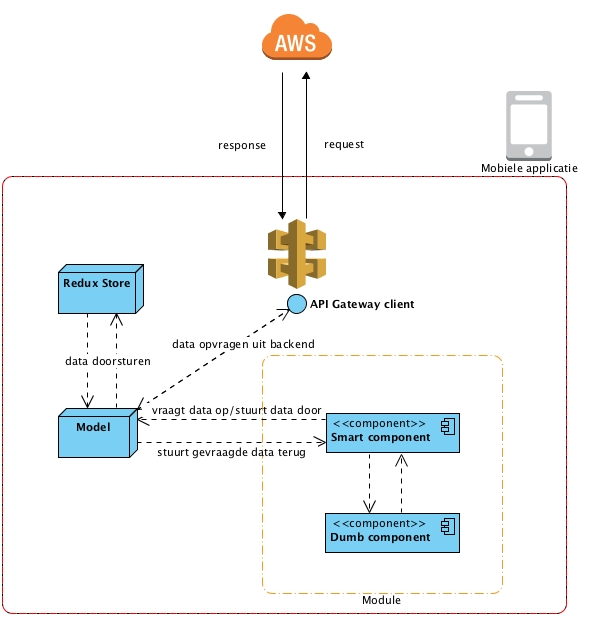
\includegraphics[width=0.9\textwidth]{mobile-overview}
\end{figure}

De applicatie maakt gebruik van verschillende design principes\autocite{brechtbilliet-scalable}\autocite{minko-gechev-scalable} die ervoor zorgen dat het een schaalbare Angular applicatie is. De applicatie bestaat uit verschillende Angular modules\footnote{Een Angular module is een verzameling van componenten en services. Modules organiseren een applicatie in coherente blokken van functionaliteit} die elke een feature voorstellen in de applicatie. 
\clearpage
Modules die data nodig hebben gebruiken een model\footnote{'model' verwijst in deze context naar een 'service' in Angular terminologie} voor het ophalen van de data uit de redux store. Indien de data niet in de store aanwezig is wordt die met behulp van de AWS API Gateway client opgevraagd aan de backend. De opgevraagde data wordt meteen in de store gestopt om het SSOT-principe te respecteren. Een smart component kan dan via zijn model data uit de redux store opvragen en stuurt die dan door naar een dumb component of meerdere dumb components. Wanneer er data wordt gewijzigd of gecree\"erd in een dumb component, stuurt het component de data terug naar zijn parent smart component. Via het model van de smart component wordt er in de store een nieuwe state gecree\"erd op basis van de nieuwe of aangepaste data.

Er wordt momenteel geen rekening gehouden met het cachen en precachen van data indien de applicatie plots offline is. Dit komt wel aan bod in het hoofdstuk ~\ref{ch:onderzoek} 'Onderzoek'
\section{Server}
De backend is opgebouwd volgens het 'serverless'\autocite{scalable-theorie} principe. Hierbij vormen AWS Lambda's de ruggengraat van de backend infrastructuur. Er wordt gebruik gemaakt van verschillende microservices die elk een beperkte maar specifieke verantwoordelijkheid hebben over een bepaalde functionaliteit. Voor de persistentie van de data wordt per data 'type'\footnote{Bijvoorbeeld pati\"enten en observaties zijn 2 verschillende datatypes} een DynamoDB tabel gebruikt. Met behulp van SNS kunnen Lambda's of andere AWS services op de hoogte worden gebracht wanneer er een neveneffect moet optreden bij het afhandelen van een request. De API Gateway is de toeganspoort tot de backend en is verantwoordelijk voor het delegeren van de binnenkomende requests. In de business case wordt er gebruik gemaakt van een proxy\footnote{Wanneer een lambda met proxy integration wordt gebruikt, hanteert de API Gateway een greedy 'catch-all' principe. Hierbij worden alle requests opgevangen en doorgestuurd naar de proxy lambda} lambda die de requests mapped naar de correcte lambda. Die voert dan de noodzakelijke stappen uit voor de request te verwerken.

\begin{figure}[h]
\label{fig:serverless}
\caption{Voorbeeld van een serverless architectuur opgezet met verschillende Amazon Web Services}
\centering
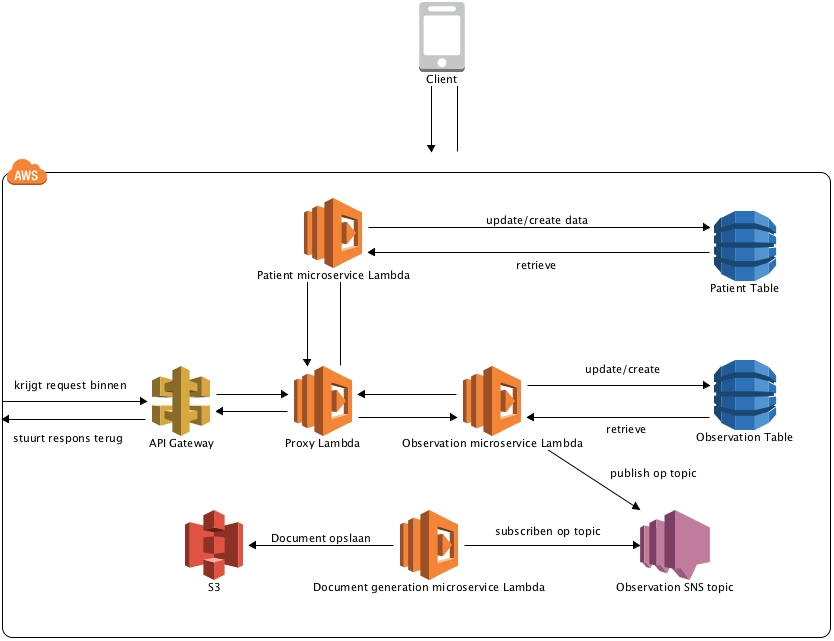
\includegraphics[width=0.9\textwidth]{serverless-example}
\end{figure}

Figuur~\ref{fig:serverless} is een voorbeeld van verschillende lambda's waarbij manipulaties worden uitgevoerd op patient -en observatiedata. De API Gateway stuurt een request naar de proxy lambda. Die triggert op zijn beurt de relevante lambda. Wanneer er een aanpassing gebeurt in de observatie data, plaatst de observatie microservice lambda een bericht op een SNS topic. Dit triggert dan de documentatie lambda die subscribed is op het SNS topic. Lambda en SNS werken dus perfect in tandem in het kader van een event-driven architectuur. 
%%=============================================================================
%% Synchronisatie methodes
%%=============================================================================

\chapter{Synchronisatie patterns}
\label{ch:synchronisatiemethdodes}

%% Bespreken synchronisatie patterns

In dit hoofdstuk worden enkele synchronisatie methodes en technieken besproken die data kan synchroniseren met de databank. Indien van toepassing, wordt telkens een concrete situatie van de use case van Pridiktiv gebruikt ter illustratie. Op het einde van dit hoofdstuk worden ook nog andere technieken besproken die niet meteen kunnen worden onderverdeeld onder een specifiek pattern.

\section{Read-Only Data}
Dit data synchronisatie patroon wordt gebruikt wanneer de end user enkel maar data moet kunnen opvragen terwijl de applicatie offline is en die data niet hoeft te manipuleren of de manipulaties op die data niet belangrijk genoeg zijn om te persisteren. Bij Read-Only Data is de richting van het dataverkeer unidirectioneel, van server naar end-user applicatie. Het Read-Only pattern hanteert volgende logica:
\begin{enumerate}
\item De end-user (client) vraagt de data op van de server. De server is de SSOT en houdt alle data bij. Die data kan wijzigen wanneer de end-user bijvoorbeeld offline is.
\item Server retourneert de data. De opgevraagde data wordt lokaal opgeslagen.
\item Alle manipulaties op de data worden geblokkeerd en worden nooit doorgegeven aan de server. De client kan dus enkel maar GET HTTP requests sturen voor de data op te vragen.
\item Bij synchronisatie wordt de oude data lokaal verwijderd en vervangen door de nieuwe data.
\item De applicatie controleert op regelmatige tijdstippen of de data is gewijzigd.
\end{enumerate}
Een voorbeeld van het Read-Only pattern van in de use case van Pridiktiv is het opvragen van de pati\"entenlijst. Die lijst kan worden gewijzigd door de hoofdverpleger in het dashboard maar niet in de applicatie zelf. Wanneer de applicatie offline is, kan eenvoudig worden verder gewerkt met de applicatie. Indien er een nieuwe pati\"ent wordt toegevoegd, dan is die vanaf de volgende synchronisatie zichtbaar.
\section{Read-Only Data Optimized}
Het Read-Only Data Optimized pattern is identiek aan het Read-Only Data pattern maar met 1 verschil. Bij de synchronisatie wordt enkel de data opgevraagd die gewijzigd is en niet alle data. Dit kan op verschillende manieren worden ge\"implementeerd. Er kan een timestamp worden bijgehouden van de laatste wijziging of een version number die incrementeert bij elke wijziging. Op basis van de vergelijking tussen de bestaande data en de data op de databank, kan de applicatie al dan niet beslissen om de lokale data te updaten. De richting van het dataverkeer is bidirectioneel, wat ook verschilt met de standaard implementatie van het Read-Only pattern. Omdat de server eerst moet worden gevraagd of er al dan niet data is gewijzigd, moet de applicatie ook kunnen communieren met de server.
\section{Read/Write Data Last Write Wins}
In dit pattern gaat de server er van uit dat writes altijd in de juiste volgorde worden uitgevoerd en de laatste write die naar de databank wordt gestuurd ook de werkelijke laatste wijziging is van de client applicatie. Er wordt geen conflict resolution uitgevoerd. Het pattern blinkt uit wanneer er enkel wordt toegevoegd en de data nooit wordt gemanipuleerd. In de use case van Pridiktiv kan dit worden toegepast bij bijvoorbeeld het toevoegen van notities bij een patient. De notities van een patient worden niet gewijzigd waardoor er geen data kan worden overschreven.
\section{Read/Write with Conflict Detection}
Het Read/Write with Conflict Detection pattern is het meest complexe waarbij verschillende end-users de dezelfde data wijzigen op het moment dat de applicatie offline is. Bij dit pattern wordt er gesproken van multi-way synchronisatie waarbij een applicatie zowel de data van de server kan updaten en dat de server op zijn beurt alle andere apparaten moet updaten. Een mogelijke flow van het proces zou er als volgt kunnen uitzien:
\begin{enumerate}
\item De server database houdt alle data bij
\item De applicatie houdt lokaal een subset van de data bij die kan worden gewijzigd.
\item Bij synchronisatie wordt de aangepaste data die lokaal wordt opgeslagen naar de server en omgekeerd.
\item In de server wordt de data aangepast en alle conflicting changes worden geregistreerd voor verdere behandeling
\item Vraagt de gebruiker voor conflict resolution of de applicatie kan zelf het conflict oplossen en de data aanpassen.
\end{enumerate}
Een voorbeeld uit de use case van Pridiktiv die gebruik zou kunnen maken van het Read/Write with Conflict Resolution pattern is de opvolging bij wondzorg. Wanneer een end-user een bepaalde wijziging aanbrengt in het dossier van de patient, is het belangrijk dat die data niet verloren gaat indien een andere end-user ook het wondzorg dossier van een patient aanpast. Het is belangrijk om conflict resolution 'achter de schermen' op te lossen om op die manier ervoor te zorgen dat er geen aanpassingen verloren gaan.

%%=============================================================================
%% Onderzoek
%%=============================================================================

\chapter{Onderzoek}
\label{ch:onderzoek}

In dit hoofdstuk wordt dieper ingegaan op de verschillende methodes  en de real-world toepassing van die methodes met de testopstelling en de businesscase. De invalshoek voor dit onderzoek is steeds een statusverandering van offline naar online.Volgende methodes komen aan bod:
\begin{itemize}
\item Read-only Optimised
\item Last/First Write Wins
\item Conflict resolution
\end{itemize}

\section{Online/Offline status registratie}
Voor bovenstaande synchronisatie methodes worden besproken is het belangrijk om aan te geven welke methode er wordt gebruikt zodat de applicatie kan waarnemen dat die al dan niet online is. Er zijn 2 mogelijkheden:
\begin{enumerate}
\item DOM API's aanspreken vanuit JavaScript: helaas is er geen consistente crossbrowser support op het controleren van de status van de verbinding zonder gebruik te maken van van requests naar externe data. Bijvoorbeeld luisteren naar events van het document.window object om online en offline status te controleren werkt niet op alle browsers. Een andere optie waarbij de status van de verbinding wordt opgevraagd met window.navigator.onLine werkt ook niet consistent in alle browsers.
\item Een request uitvoeren naar een externe bron: als de applicatie een request uitvoert naar een externe bron en de HTTP code controleert van de respons, dan kan de applicatie gemakkelijk afleiden wat de status van de verbinding is. Deze methode garandeert dat de applicatie correct kan vaststellen wanneer de status van de verbinding verandert. Deze methode ook gebruikt in libraries zoals Offline.js.
\end{enumerate}

\begin{lstlisting}[caption=DOM API's voor controleren offline en online status]
    // FIREFOX met jQuery
    $(window).bind("online", applicationBackOnline); 
    $(window).bind("offline", applicationOffline);

    //IE met vendor specifieke objecten
    window.onload = function() {
        document.body.ononline = ConnectionEvent;
        document.body.onoffline = ConnectionEvent;
    }
    
    // met window.navigator
    if (navigator.onLine) {
  	// Online
     } else {
  	// Offline
	}
    
\end{lstlisting}

\subsection{Gecachte data doorsturen naar de server}
Voor het onderzoek werd geopteerd op gebruik te maken van de tweede methode. Wanneer de applicatie registreert dat er geen verbinding meer is, worden alle requests gecached als afzonderlijke objecten. Wanneer de applicatie dan terug online is, wordt er in een request naar de server alle gecachte data doorgestuurd. De API Gateway geeft het object door aan een gateway lambda die de objecten op een queue plaatst.  Een andere lambda leest alle boodschappen uit de queue en stuurt elke request terug naar de gateway lambda. De API Gateway wijst de correcte lambda aan die verantwoordelijk is voor de verwerking van de oorspronkelijke request. Bij requests die een UPDATE uitvoeren op een object dat aangemaakt werd (CREATE) tijdens de offline status, worden allemaal gebundeld in een object. Op die manier wordt de volgorde gegarandeerd voor het verwerken van de verschillende requests. Wanneer er dan synchronisatieproblemen optreden, moeten die in de lambda's worden opgevangen die de individuele request moeten verwerken.

\section{Data caching uit backend}
Bij een applicatie die zowel online als offline moet werken, is het belangrijk dat er data wordt gepreload in de applicatie. Zo kan de gebruiker blijven verder werken indien de applicatie plots offline zou zijn. Het belangrijkste aandachtspunt is hierbij de schaalbaarheid van de oplossing. In de business case van Pridiktiv worden verschillende requests naar de server uitgevoerd naar de server om de data op te vragen. Wanneer de functionaliteit en data capaciteit van de applicatie toeneemt kan het aantal requests kan wel dramatisch stijgen. Een mogelijke oplossing voor dat probleem kan een webworker zijn. Door het single-threaded karakter van JavaScript kan er een webworker worden gebruikt voor het parallel bevragen van de server.

De connectie status van de de applicatie wordt bewaard als state in de ngrx store. Die kan worden bevraagd bij het uitvoeren wanneer er data uit de store moet worden geladen. Zo weet de applicatie of het al dan niet mogelijk is om een request naar de server uit te voeren. De ngrx store is de SSOT en bevat die de gecachte data in-memory. Wanneer de store wordt bevraagd kan de gecachte data uit de store worden geladen. Dit laat de gebruikers toe om zonder onderbreking de applicatie te gebruiken wanneer er verandering in de verbindingsstatus is.

\subsection{Beperkingen door single-threaded omgeving}
JavaScript is een single-threaded omgeving waardoor meerdere scripts niet simultaan kunnen worden uitgevoerd. Dit vormt problemen wanneer een webapplicatie UI events, queries, een groot volume API data en tegelijk de DOM aanpassingen moet verwerken. Met technieken zoals setTimeout() en setInterval() is het mogelijk om concurrency te simuleren maar dit maakt de applicatie meteen een stuk complexer. Dankzij de HTML5 specificatie is het mogelijk om Web Workers te gebruiken. Deze laten toe om scripts in de achtergrond uit te voeren. Hierdoor is het mogelijk om complexe berekeningen concurrent uit te voeren zonder dat dit een performantie impact op de applicatie heeft.

\subsection{Toepassing op prototype}
In het onderzoek zijn twee verschillende mogelijkheden voor caching onderzocht. De eerste methode vraagt serieel alle data op van de server. Dit vormt geen probleem indien de data beperkt is, maar eenmaal het volume van de data stijgt, dan moeten er steeds meer requests wordt uitgevoerd naar de server. Dit heeft als nadeel dat de main thread geblocked wordt waardoor er geen UI kan worden gerenderd op het toestel. Dit is dus geen ideaal scenario. Bij de andere 2 methodes wordt er gebruik gemaakt van een webworker. Deze webworker laat doe om parallel met de applicatie bepaalde acties uit te voeren. Met behulp van de webworker is het dan mogelijk om de caching in de achtergrond uit te voeren. Met deze web workers kunnen dan volgende operaties worden uitgevoerd:

\begin{enumerate}
\item data ophalen van de server
\item omzetten van opgehaalde data naar state object voor ngrx
\end{enumerate}

Om het aantal requests drastisch te verminderen is het ook mogelijk om bepaalde data te bundelen. Zo kunnen alle observaties voor patienten worden gebundeld worden in 1 object en de webworker vormt die response dan om naar een geldig state object. Zo worden intensieve berekeningen in de applicatie vermeden. Een andere mogelijkheid is het opzetten van een applicatie state in de backend en dit dan door te sturen. Op die manier moet enkel het state object worden toegevoegd aan de store wanneer het is opgevraagd van de server. een nadeel van deze methode is de state van de client die nu sterk gekoppeld is aan de backend.

\subsection{Toepassing op de business case}
In de business case wordt de request serieel bevraagd van de server. Nadat de pati\"entenlijst is opgevraagd, worden voor alle pati\"enten de relevante data opgevraagd. In de piloot versie waren dat ongeveer 75 personen die elk taken, notities, observaties, medische parameters en wondzorgdossiers kunnen bevatten. Dit leidt tot een 500 requests die in een zeer korte periode worden uitgevoerd. Het gebruik van web workers \autocite{webworker-reference} gecombineerd met een gebundelde data zou het aantal requests sterk kunnen verminderen. In de business case is er ook sprake van afbeeldingen die moeten worden gesynchroniseerd met de applicatie maar het cachen van BLOBs valt buiten de scope van dit onderzoek.

\section{Data synchronisatie: planning bij development}
Wanneer een synchronisatieoplossing moet worden ontwikkeld voor een applicatie, is het belangrijk om alle use cases in kaart te brengen waarbij er rekening moet worden gehouden met synchronisatie. Dit zorgt ervoor dat er geen functionaliteit over het hoofd wordt gezien bij het ontwikkelen van de synchronisatieoplossing. Ter illustratie wordt in de onderstaande voorbeeld de business case van Pridiktiv ontleed.

\section{Data synchronisatie: planning bij development}
Wanneer een synchronisatieoplossing moet worden ontwikkeld voor een applicatie, is het belangrijk om alle use cases in kaart te brengen waarbij er rekening moet worden gehouden met synchronisatie. Dit zorgt ervoor dat er geen functionaliteit over het hoofd wordt gezien bij het ontwikkelen van de synchronisatieoplossing. Ter illustratie wordt in de onderstaande voorbeeld de business case van Pridiktiv ontleed.

\begin{center}
    \begin{tabular}{ l | r }
    \hline
    Functionaliteit & Synchronisatie \\ \hline
    Taken & First-Write Wins of conflict resolution \\
    Observaties & geen conflict mogelijk \\
    Medische data & geen conflict mogelijk \\
    Wondzorg & First-Write Wins of conflict resolution \\
    Notities & Geen conflict mogelijk \\
    \hline
    \end{tabular}
\end{center}

De onderverdeling is het uitgangspunt voor de volgende stap namelijk het bepalen van de verschillende synchronisatie mogelijkheden. Zo kan bijvoorbeeld worden bepaald dat de gebruiker bij een conflict zelf een beslissing moet nemen. Of indien er een conflict optreedt bij een synchronisatie van bepaalde data, dat er automatisch voor Last/First Write Wins wordt gekozen. In het geval waarbij er conflict resolution moet gebeuren door de gebruiker, kunnen kan worden bepaald welke keuzes de gebruiker krijgen en welke keuzes de server zelf kan maken. Bovenstaande overzicht vormt dan als het ware de basis voor de ontwikkeling van de synchronisatie. Een ander voorbeeld is het deactiveren van bepaalde functionaliteit bij wanneer de applicatie offline is. Hierdoor kunnen potentieel complexe synchronisatieproblemen worden vermeden. Dit heeft echter als nadeel dat de applicatie niet meer de volledige functionaliteit kan aanbieden wanneer de verbinding is verbroken. Het al dan niet uitschakelen van bepaalde functionaliteit bij offline gebruik is sterk afhankelijk van de business case

De onderverdeling is het uitgangspunt voor de volgende stap namelijk het bepalen van de verschillende synchronisatie mogelijkheden. Zo kan bijvoorbeeld worden bepaald dat de gebruiker bij een conflict zelf een beslissing moet nemen. Of indien er een conflict optreedt bij een synchronisatie van bepaalde data, dat er automatisch voor Last/First Write Wins wordt gekozen. In het geval waarbij er conflict resolution moet gebeuren door de gebruiker, kunnen kan worden bepaald welke keuzes de gebruiker krijgen en welke keuzes de server zelf kan maken. Bovenstaande overzicht vormt dan als het ware de basis voor de ontwikkeling van de synchronisatie. Een ander voorbeeld is het deactiveren van bepaalde functionaliteit bij wanneer de applicatie offline is. Hierdoor kunnen potentieel complexe synchronisatieproblemen worden vermeden. Dit heeft echter als nadeel dat de applicatie niet meer de volledige functionaliteit kan aanbieden wanneer de verbinding is verbroken. Het al dan niet uitschakelen van bepaalde functionaliteit bij offline gebruik is sterk afhankelijk van de business case

\section{Read-Only Optimised}
De belangrijkste insteek voor deze methode is om zo effici\"ent mogelijk gebruik te maken van de bandbreedte van de client. Read-Only Optimised is dan ook eerder een optimalisatietechniek dan een synchronisatiemethode. Deze techniek laat toe om enkel nieuwe data binnen te halen waardoor data die de client reeds bezit niet opnieuw worden opgevraagd. De complexiteit van deze methode stijgt evenredig met het aantal parameters dat in de data kan worden aangepast. Van alle methodes die in dit hoofdstuk worden besproken, is dit de enige methode waarbij enkel een HTTP GET wordt gebruikt. Deze methode is ook enkel maar belangrijk bij het caching van data voor offline en online gebruik.
\subsection{Overzicht: Client}
Bij Read-Only Optimised staat de synchronisatie van de client centraal. Tijdens de periode dat de client offline was, is het mogelijk dat er nieuwe data zijn aangemaakt. Om deze data te synchroniseren kan de client alle data opnieuw opvragen maar deze manier heeft enkele nadelen. Indien de data klein is zoals enkel tekst, dan is Read-Only Optimised triviaal en kunnen alle data opnieuw worden opgevraagd. Wanneer er echter grotere data moet worden ingeladen zoals afbeeldingen, dan kan Read-Only Optimised heel wat bandbreedte uitsparen. Dankzij de ngrx store is het ook gemakkelijk om manipulaties uit te voeren op de data, waardoor er eenvoudig objecten kunnen worden toegevoegd aan de data in de store. Belangrijke voorwaarde voor het uitvoeren van deze actie is het bijhouden in de client van de timestamp van de laatste update indien de data aanwezig zijn. Indien er geen timestamp aanwezig is, dan weet de client dat alle data moeten worden opgevraagd.

<TODO request invoegen>

Bovenstaande afbeelding is een voorbeeld van een Read-Only Optimised request waarbij enkel de nieuwe data worden aangevraagd. Wanneer de client een HTTP GET uitvoert, dan wordt in de header van de request de timestamp van de laatste update toegevoegd. Deze timestamp is belangrijk voor de verwerking server side bij voor het uitvoeren van een query op de databank.

<TOEVOEGEN SCREENSHOT USE CASE IN SETUP APPLICATIE >
De wijzigingen zijn dan meteen zichtbaar in de store en bijgevolg ook in de client.
\subsection{Overzicht: Server}
De server heeft net zoals bij een traditionele GET de verantwoordelijkheid om de data op te vragen uit de databank en die terug te sturen naar de client. Het enige verschil is dat er rekening moet worden gehouden met de een mogelijke timestamp in de header. Op basis van die timestamp kan dan alle nieuwe data sinds de laatste GET worden opgevraagd. De request wordt doorgestuurd naar 

<TOEVOEGEN VP OVERZICHT BACKEND INFRASTRUCTUUR VOOR READ-ONLY OPTIMISED>

\subsection{Opmerkingen}
Ondanks de perceptie dat dit een eenvoudige methode is, zijn er enkele opmerkingen zij deze methode:
\begin{enumerate}
\item In bovenstaand scenario wordt er enkel maar uitgegaan van nieuwe data, dus CREATE operaties. Indien de methode ook voor UPDATE moet werken is het in bepaalde gevallen noodzakelijk om ook de databank structuur aan te passen.
\item Bij klassieke SQL databanken kan gemakkelijk worden gefilterd op bepaalde velden zoals een 'updated veld' binnen een tabel. Bij DynamoDB is dit moeilijker als de waarde van de query geen deel uitmaakt van de sort -of partition key. In dat geval moet er dan gebruik worden gemaakt van een extra secondary index zodat er geen full table scan moet worden uitgevoerd telkens wanneer er een GET request is.
\item Het is bij kleine data vaak eenvoudiger om steeds alle data op te vragen en geen gebruik te maken van de Read-Only Optimised methode.
\end{enumerate}
\subsection{Toepassing op prototype}
Met behulp van een timestamp wordt er bijgehouden wanneer de laatste GET is uitgevoerd. Op die manier kan de backend bepalen welke informatie er moet worden geretourneerd. Wanneer er enkel maar eenvoudige data moet worden geretourneerd zoals JSON dan zorgt de Read-Only Optimised methode nodeloos voor extra complexiteit. Het is daarom enkel aangeraden om enkel Read-Only Optimised te gebruiken indien er met andere en grotere data wordt gewerkt.
\subsection{Toepassing op de business case}
In de backoffice en mobiele applicatie van Pridiktiv wordt er momenteel geen gebruikt gemaakt van Read-Only Optimised. Omdat synchronisatie momenteel de grootste zorg is van de organisatie, is Read-Only Optimised minder belangrijk in de business case.
\section{Last/First Write Wins}
Bij Last/First Write Wins gaat er onherroepelijk informatie verloren. Afhankelijk van de gekozen conflict resolution methode is het wordt de eerste of laatste write bijgehouden. Dit is de eenvoudigste manier van conflict resolution maar men moet bereidt zijn om een compromis te sluiten en informatie op te offeren in ruil voor minder complexiteit bij het synchroniseren. Wanneer heel snel naar een offline/online synchronisatiemethode moet worden gezocht, biedt die de gemakkelijkste oplossing.
\subsection{Overzicht: Client}
Bij deze methode is de impact van de client miniem want de client weet niet dat er een synchronisatieprobleem zal optreden wanneer die data doorstuurt naar de server.
\subsection{Overzicht: Server}
Deze methode vind plaats wanneer verschillende clients een verandering aanbrengen bij hetzelfde bestaande object. Hierdoor krijgt de databank verschillende waarden binnen en moet dat verplicht de databank er toe om te reageren. Afhankelijk van de methode die gekozen zijn er twee scenario's mogelijk bij deze synchronisatiemethode.
\begin{enumerate}
\item First Write Wins. Hier wordt enkel de eerste write van een object of row bijgehouden. Indien hetzelfde object opnieuw wordt aangepast dan wordt er een exceptie geworpen. Dit is enkel maar mogelijk in use cases waarbij een aanpassing in een object finaal is. Een voorbeeld uit de use case is bijvoorbeeld het volbrengen van een taak. Wanneer een taak is volbracht, is het niet meer mogelijk om die aan te passen. Met behulp van een completed flag kan de state van de taak worden bijgehouden. Wanneer de aanpassingen in een object niet finaal zijn, is een last Write wins een betere methode.
\item Last Write Wins. Bij Last Write Wins wordt enkel maar de laatste write operatie behouden. Er wordt geen vergelijking gemaakt met de waarde die reeds in de databank beschikbaar is en de nieuwe waarde die wordt doorgegeven. Men hanteert deze methode dan best enkel bij bestaande objecten waarbij het mogelijk is om UPDATE operaties op uit te voeren.
\end{enumerate}
\subsection{Opmerkingen}
First/Last Write wins is een aantrekkelijke methode wanneer er op korte termijn synchronisatie moet worden gerealiseerd maar er zijn wel enkele bemerkingen bij deze methode.
\begin{itemize}
\item Er gaat onherroepelijk data verloren op deze manier. Indien de use case dit niet toelaat dan moet er worden gekeken naar andere conflict resolution policy.
\item Het type van de data (finaal of niet-finaal) sluit de andere methode uit. Niet-finale data met First Write Wins maken de data impliciet finaal en immutable.
\end{itemize}
\subsection{Toepassing op prototype}
Deze synchronisatiemethode is de meest eenvoudige en wordt in het prototype gedemonstreerd aan de hand van twee scenario's in de client.
\begin{enumerate}
\item Er worden taken volbracht. Die zijn finaal en worden dus verwerkt volgens de First Write Wins
\item Een notitie wordt gewijzigd. Hier geldt de Last Write Wins regel want een notitie aanpassen is nooit finaal.
\end{enumerate}
\subsection{Toepassing op de business case}
Momenteel hanteert de backend van Pridiktiv enkel een First/Last Write principe bij data. Naar de toekomst zou dit moeten veranderen naar een een bredere oplossing die conflict resolution kan aanbieden.
\section{Conflict Resolution}
Bij synchronisatie gaat er idealiter geen informatie verloren of laat de business case gaan dataverlies toe. Daarom is het ook belangrijk om te kijken hoe data kan worden gesynchroniseerd op een manier waarbij geen data verloren gaan. Om het onderzoek binnen de restricties van de business case te laten passen, worden hier enkel AWS services gebruikt bij het synchronisatie. Een andere belangrijke opmerking dat het enkel maar gaat over UPDATE en DELETE operaties want Een CREATE operatie kan niet leiden tot een conflict wanneer het toestel offline is.
\subsection{Overzicht: Client}
Net zoals bij First/Last Write Wins, is de rol van de client beperkt. Wanneer de data zonder timestamp in de database wordt bewaard, is het belangrijk om een timestamp bij te houden wanneer nieuwe data zijn aangemaakt of aangepast. Zo heeft de server een referentiepunt om de data te verwerken.
\subsection{Overzicht: Server}
Timestamps bieden een eenvoudige oplossing om de controleren wanneer een bepaalde actie heeft plaatsgevonden. De timestamp van het nieuwe aangepaste object wordt vergeleken met de timestamp van het object dat reeds aanwezig is in de database. Zo kan bijvoorbeeld een timestamp worden bijgehouden in een 'modified' veld. Dat veld kan worden vergeleken met de timestamp van de UPDATE of DELETE die wordt doorgestuurd. Zo kan de server bepalen of er al dan niet een conflict is en wat er in het geval van een conflict moet gebeuren. Indien er geen timestamp sinds de laatste update wordt bewaard in het object, dan wordt synchroniseren zeer moeilijk en is First/Last Write Wins een betere oplossing. Het bijhouden van een timestamp alleen is echter niet voldoende. Het is belangrijk om op voorhand te bepalen wat de conflict resolution policies zijn en welke uses cases er allemaal van toepassing zijn. Niet alle conflicten kunnen worden opgevangen door de server. Zo kan de server geen beslissing nemen wanneer een DELETE actie wordt uitgevoerd op een object en er na nog een update wordt doorgestuurd. De gebruiker moet dan een waarschuwing krijgen dat zijn object is verwijderd en dan zijn aanpassingen niet zijn opgeslagen. Indien de gebruiker geen boodschap zou krijgen, dan wekt de server de perceptie dat er iets fout is gegaan bij de verwerking van de data.
\subsection{Toepassing op prototype}
TODO
\subsection{Toepassing op de business case}
\subsubsection{UPDATE operatie}
Pridiktiv maakt gebruik van DynamoDB voor het bijhouden van de data. In DynamoDB wordt er gewerkt met een Partition Key die kan worden vergeleken met een Primary Key in SQL-terminologie en optioneel een Sort Key die  de Partition Key bevat in combinatie met een attribuut van het object. Daarnaast is het ook nog mogelijk om Secondary Indices te cre\"eren die functioneren zoals Sort keys.  Het is belangrijk dat de timestamp de Partition Key is of deel uitmaakt van de samengestelde Sort Key. Indien niet, is de DynamoDB verplicht om een full table scan uit te voeren op de tabel en over die data set te filteren. Omdat de timestamp deel uitmaakt van de Primary Key, is het bij updates eenvoudig om bij te houden wanneer de laatste update is uitgevoerd en om te voorkomen dat een UPDATE gedupliceerd wordt. Dit laatste wordt vermeden doordat de Partition Key unique moet zijn en dus met andere woorden kan die niet worden gedupliceerd zonder dat DynamoDB een exceptie gooit.
\subsubsection{DELETE operatie}
Het is in de business case van Pridiktiv niet mogelijk om date te verwijderen. Alle data moet zichtbaar blijven in een historiek. Hierdoor is het niet toegelaten om DELETE operaties uit voeren, enkel UPDATE operaties. 
\section{Open-source libraries}
Voor het synchroniseren van de data bij Pridiktiv in AWS wordt er gebruik gemaakt van twee verschillende Open Source libraries. Deze zijn gemaakt om een oplossing aan te bieden voor Pridiktiv en in kader van dit onderzoek. De componenten zijn geschreven in JavaScript voor NodeJS 4.3 en hoger. Hierdoor is het mogelijk om nieuwere features uit ES6 te gebruiken zoals Promises. Het is specifiek ontwikkeld om te werken met Simple Queue Service van AWS maar biedt de flexibiliteit om gebruikt te worden buiten AWS Lambda, bv in AWS EC2 instances die ook NodeJS gebruiken. Deze libraries zijn ontwikkeld in kader van dit onderzoek en worden gebruikt binnen de productieomgeving van de Pridiktiv applicaties.
\subsection{aws-sqs-push}
Deze library heeft een functie die berichten op de SQS queue plaatst en een Promise retourneert wanneer er een bericht op de queue is geplaatst. De naam van de queue wordt met een hulpfunctie aws-sqs-geturl opgevraagd. Op deze manier is de gebruiker van deze library niet verplicht om de volledige ARN naam van de SQS door te geven. Wanneer de mesage een object bevat is dan wordt het object met JSON.stringify() automatisch omgevormd naar een string.

\begin{lstlisting}[caption=Voorbeeld dat data plaatst op een SQS queue met behulp van de aws-sqs-push library]

	const sqsPush = require('aws-sqs-push');

	sqsPush('QueueName', 'SomeMessage').then(messageId => {
    		console.log(messageId);
    	//=> '8a98f4d0-078b-5176-9af2-bbd871660ecb'
	});

	sqsPush('QueueName', 'SomeMessage', {awsAccountId: '123456789101'}).then(messageId => {
    		console.log(messageId);
    	//=> '8a98f4d0-078b-5176-9af2-bbd871660ecb'
	});
	
\end{lstlisting}
\clearpage
\subsection{aws-sqs-poll}
De aws-sqs-poll library vraagt aan de SQS queue berichten. Die worden dan geretourneerd als een string of indien het een stringified object is, als een object. Net zoals bij de aws-sqs-push wordt er gebruikt gemaakt van een hulplibrary voor het opvragen van de ARN naam van de queue.

\begin{lstlisting}[caption=Voorbeeld hoe berichten worden opgehaald van de SQS queue]

	const awsSqsPoll = require('aws-sqs-poll');

	awsSqsPoll('QueueName')
    	//  ["MessageId": "28f61fd2-b9ca-4cb9-879a-71ea8bce4636",
    	//   "ReceiptHandle": "AQEB9mnsxtAZlwnDERxn3yADAP96QRe0KPbqaKXLvvchqmD4jAr",
    	//   "MD5OfBody": "098f6bcd4621d373cade4e832627b4f6",
    	//   "Body": "test"]


	awsSqsPoll('QueueName', {AwsAccountId: '123456789012', numberOfMessages: 1, timeout: 20, json: false})
  	  //  ["MessageId": "28f61fd2-b9ca-4cb9-879a-71ea8bce4636",
    	//   "ReceiptHandle": "AQEB9mnsxtAZlwnDERxn3yADAP96QRe0KPbqaKXLvvchqmD4jAr",
    	//   "MD5OfBody": "098f6bcd4621d373cade4e832627b4f6",
    	//   "Body": "test"]
	
\end{lstlisting}

\subsection{aws-sqs-deletemessage}
Een kleine functie die SQS messages verwijderd op basis van de ReceiptHandle die wordt meegestuurd wanneer er een bericht wordt opgevraagd. De message is verwerkt dan mag het bericht zonder problemen worden verwijderd van de queue. Net zoals bij de andere bovenstaande functies, heb je altijd de ARN naam nodig van de SQS queue die je wenst op te roepen. Dus hier wordt opnieuw de hulpfunctie aws-sqs-geturl nodig.

\begin{lstlisting}[caption=Voorbeeld hoe een bericht wordt verwijderd van SQS nadat het is verwerkt]

	const awsSqsDeletemessage = require('aws-sqs-deletemessage');

	awsSqsDeletemessage('somequeue', 'SasuWXPJB+CwLj1FjgXUv1uSj1gUPAWV66FU/').then(id => {
		console.log(id);
		//=> 'b5293cb5-d306-4a17-9048-b263635abe4
	});

	awsSqsDeletemessage('somequeue', 'SasuWXPJB+CwLj1FjgXUv1uSj1gUPAWV66FU/', {awsAccountId: '123456789012'}).then(id => {
		console.log(id);
	//=> 'b5293cb5-d306-4a17-9048-b263635abe4
});
	
\end{lstlisting}

\subsection{aws-sqs-geturl}
Hulplibrary die de ARN naam opvraagt van een specifieke SQS queue. Aan de hand van de AWS root account id, die automatisch wordt meegestuurd in een request, kan samen met de naam de ARN naam van een bepaalde SQS queue worden opgehaald. De AWS JavaScript SDK laat dit ook toe maar de functie gebruikt callbacks en een complexere configuratie. Door het gebruik van deze hulplibrary is de configuratie verwaarloosbaar en wordt er geen gebruik gemaakt van callbacks maar van promises

\begin{lstlisting}[caption=Voorbeeld hoe de ARN van een SQS wordt opgehaald]

	const awsGetSqsUrl = require('aws-sqs-geturl');

	awsGetSqsUrl('somequeue').then(url => {
		console.log(url);
		//=> https://sqs.eu-west-1.amazonaws.com/123456789111/somequeue
	});

	awsGetSqsUrl('anotherqueue', {awsAccountId: '123456789012'}).then(url => {
		console.log(url);
	//=> https://sqs.us-west-1.amazonaws.com/123456789012/anotherqueue
	});
	
\end{lstlisting}



%% Voeg hier je eigen hoofdstukken toe die de ``corpus'' van je bachelorproef
%% vormen. De structuur en titels hangen af van je eigen onderzoek. Je kan bv.
%% elke fase in je onderzoek in een apart hoofdstuk bespreken.

%%=============================================================================
%% Conclusie
%%=============================================================================

\chapter{Conclusie}
\label{ch:conclusie}

%% TODO: Trek een duidelijke conclusie, in de vorm van een antwoord op de
%% onderzoeksvra(a)g(en). Wat was jouw bijdrage aan het onderzoeksdomein en
%% hoe biedt dit meerwaarde aan het vakgebied/doelgroep? Reflecteer kritisch
%% over het resultaat. Had je deze uitkomst verwacht? Zijn er zaken die nog
%% niet duidelijk zijn? Heeft het ondezoek geleid tot nieuwe vragen die
%% uitnodigen tot verder onderzoek?

Afhankelijk van de restricties waarbinnen een applicatie moet worden gebouwd, kan men voor online/offline synchronisatie gebruik maken van de een volledig oplossing waarbij synchronisatie wordt aangeboden als een deel van totaal pakket zoals Microsoft Azure Applications of CouchDB. De synchronisatie gebeurt hier quasi volledig automatisch. Deze opties werden maar kort toegelicht tijdens dit onderzoek. Een allesomvattende oplossing is echter niet geschikt voor elke use case. In het voorbeeld van Pridiktiv is de nood aan een managed database en het gebruik van een serverless arcitectuur met AWS Lambda's de belangrijkste redenen om zelf de synchronisatie methodes in te bouwen in de huidige applicatie.

Wanneer online/offline synchronisatie moet worden ge\"implementeerd in een applicatie,  bestaat de eerste stap om de use cases onder te verdelen in de verschillende manieren voor synchronisatie. Wanneer absoluut geen data mag verloren gaan moet men resoluut kiezen voor conflict resolution. Wanneer niet alle data belangrijk is, kan er worden geopteerd voor een First/Last Write Wins techniek waarbij er onherroepelijk informatie verloren gaat. De belangrijkste conclusie die men uit het onderzoek kan trekken is dat er geen allesomvattende methode bestaat maar eerder een verzameling aan technieken op om synchronisatie van data uit de client en server te waarborgen. Wanneer synchronisatie wordt ingebouwd is het belangrijk om ook rekening te houden met performantie en effici\"entie en om de verantwoordelijkheid te verdelen tussen client -en server side.

Een interessante piste voor Amazon is dan ook zonder twijfel een service waarbij data uit mobiele applicaties of andere externe data sources gesynchroniseerd wordt met DynamoDB (of Aurora, een andere managed databank die Amazon Web Services aanbiedt).

%%---------- Back matter ------------------------------------------------------

\printbibliography
\addcontentsline{toc}{chapter}{\textcolor{maincolor}{\IfLanguageName{dutch}{Bibliografie}{Bibliography}}}

\listoffigures
\listoftables

\end{document}
